\chapter{Selective Reagent Ion Mass Spectrometric Investigations of the Nitroanilines}\label{chapter:nas}
\markboth{Nitroanilines in SRI-MS}{}


This chapter is a reformatted copy of my published article (reference \cite{nitroanilinespaperreference}):

\fullcite{nitroanilinespaperreference}.








\section*{Declaration of contribution}
My contribution to the article of which the present chapter is composed of was 
performing the experiments, analysing the results and writing the manuscript together with the coauthors. 
The DFT calculations used to aid in the interpretation of the data were made by Dr Peter Watts (Molecular Physics Research Group, University of Birmingham).








\section{Abstract}
This paper presents an investigation of proton and charge transfer reactions to 2-, 3- and 4-nitroaniline (C$_6$H$_6$N$_2$O$_2$) involving the reagent ions H$_3$O$^+$.(H$_2$O)$_n$ (n = 0, 1 and 2) and O$_2^+$, respectively, as a function of reduced electric field (60-250 Td), using Selective Reagent Ion – Time-of-Flight – Mass Spectrometry (SRI-ToF-MS). To aid in the interpretation of the H$_3$O$^+$.(H$_2$O)$_n$ experimental data, the proton affinities and gas-phase basicities for the three nitroaniline isomers have been determined using density functional theory. These calculations show that proton transfer from both the H$_3$O$^+$ and H$_3$O$^+$.H$_2$O reagent ions to the nitroanilines will be exoergic and hence efficient, with the reactions proceeding at the collisional rate. For proton transfer from H$_3$O$^+$ to the NO$_2$ sites, the exoergicities are 171 kJ mol$^{-1}$ (1.8 eV), 147 kJ mol$^{-1}$ (1.5 eV), and 194 kJ mol$^{-1}$ (2.0 eV) for 2-, 3- and 4-nitroaniline, respectively. Electron transfer from all three of the nitroanilines is also significantly exothermic by approximately 4 eV. Although a substantial transfer of energy occurs during the ion/molecule reactions, the processes are found to predominantly proceed via non-dissociative pathways over a large reduced electric field range. Only at relatively high reduced electric fields (> 180 Td) is dissociative proton and charge transfer observed. Differences in fragment product ions and their intensities provides a means to distinguish the isomers, with proton transfer distinguishing 2-NA from 3- and 4-NA, and charge transfer distinguishing 4-NA from 2- and 3-NA, thereby providing a means to enhance selectivity using SRI-ToF-MS.

\textbf{\textit{Keywords}}: Soft Chemical Ionisation-Mass Spectrometry; Proton Transfer Reaction Mass Spectrometry; Nitroanilines; Explosives; Charge transfer. 




\section{Introduction}
\acrfull{srims} is a variation of the soft chemical ionisation technique  PTR-MS that uses not only H$_3$O$^+$ but also other reagent ions, like O$_2^+$ and NO$^+$, that undergo charge transfer with the analyte rather than proton transfer \cite{ellis2013proton}.
It has been proved an useful tool in several fields, like the environmental sciences, food sciences, atmospheric chemistry, health science and homeland security \cite{biasioli2011direct,mayhew2010applications,sulzer2012proton,kassebacher2013investigations,FERNANDEZDELRIO20151243,trefz2018effects,herbig2014towards,ruzsanyi2018breath,Agarwal2011,lanza2015selective,critchley2004proton}.  
Like PTR-MS, SRI-MS is used to investigate ion/molecule reactions occuring inside a drift tube maintained at a known pressure, temperature, humidity and collisional energy. 
Then analyte molecules of interest are introduced through the inlet pipe (typically without pre-separation) into the drift tube, where they meet the reagent ions, and the proton or charge transfer reaction occurs. 
The switching between the different reagent ion species can be done quick enough ($\sim$100 ms), which makes SRI-MS a suitable tool for transient experiments.  
%Here we present a study of the reactions of three nitroaniline isomers with both O$_2^+$ and H$_3$O$^+$ as a function of the reduced electric field.



%\acrfull{srims} is a commonly used soft chemical ionisation technique used in a broad range of analytical fields and applications \cite{ellis2013proton,biasioli2011direct}. These include environmental analysis, food science, atmospheric chemistry, health science, homeland security, and breath analysis \cite{mayhew2010applications,sulzer2012proton,kassebacher2013investigations,FERNANDEZDELRIO20151243,trefz2018effects,herbig2014towards,ruzsanyi2018breath,Agarwal2011,lanza2015selective,critchley2004proton}.  Its analytical technique is based on ion/molecule reactions in a controlled environment, namely a drift tube maintained at a constant pressure, temperature, humidity and fixed electric field. Commonly used reagent ions are H$_3$O$^+$ and O$_2^+$, which react with traces of neutral organic molecules, injected directly into the drift tube of the instrument, usually with no pre-separation step. This allows for real-time analysis with a time resolution of approx. 100 msec. These attributes make SRI-MS an ideal technique for detecting compounds that are only transiently (seconds) present in the drift tube. When H$_3$O$^+$ is only used as the reagent ion, the technique is better known as Proton Transfer Reaction-Mass Spectrometry (PTR-MS) \cite{ellis2013proton}. In this study, we investigated reactions involving both O$_2^+$ and H$_3$O$^+$, and hence the term SRI-MS is more appropriate for the work presented here. 

Over the last few years, many projects have been conducted to confirm the applicability of SRI-MS to Homeland Security \cite{mayhew2010applications,sulzer2012proton,kassebacher2013investigations,RN445,shen2009triacetone,jurschik2010proton,sulzer2013applications,agarwal2014sensitivity,RF_TNT,gonzalez2017development,doi:10.1021/acs.analchem.7b05211,doi:10.1002/rcm.4334,gonzalez2019applications}.  
The main achieved goals are the development of instrumentation and the improvement of our understanding of the ion/molecule reactions happening in the drift tube.
The former includes the use of different reagent ions \cite{RN1254}, new sampling methods \cite{RN445}, implementation of radio frequency ion funnels  \cite{RF_TNT,barber2012increased} and rapid electric field switching \cite{doi:10.1021/acs.analchem.7b05211}. 
%During the last 10 years a large amount of work exploring the capabilities of SRI-MS for Homeland Security has been undertaken \cite{mayhew2010applications,sulzer2012proton,kassebacher2013investigations,RN445,shen2009triacetone,jurschik2010proton,sulzer2013applications,agarwal2014sensitivity,RF_TNT,gonzalez2017development,doi:10.1021/acs.analchem.7b05211,doi:10.1002/rcm.4334,gonzalez2019applications}. Two key objectives of this work are the following: (i) instrumental development for enhancing SRI-MS analytical performance (such as use of different reagent ions \cite{RN1254}, new sample inlet methods \cite{RN445}, use of ion funnel for either enhanced sensitivity or selectivity \cite{RF_TNT,barber2012increased}, and fast reduced electric field switching for enhanced selectivity \cite{doi:10.1021/acs.analchem.7b05211}); and (ii) improving our knowledge of the underlying ion/molecule chemistry occurring within the reagent region of the analytical device.
One of the drawbacks of SRI-MS is that %this technique is that %in most cases 
it is not possible to directly distinguish between isomeric compounds, although there are  exceptions  \cite{lanza2013distinguishing}. 
Here we present a study of the reactions of three nitroaniline (NA) isomers with both O$_2^+$ and H$_3$O$^+$ as a function of the reduced electric field. The main goal is to determine if they can be distinguished without initial pre-separation by solely enhancing the ion/molecule reactions using different reagent ions.



%A limitation with the selectivity of SRI-MS is associated with its capability to distinguish isomers. This is particularly true for proton transfer reactions, where often only the protonated parent\footnote{Although revised IUPAC recommendations for terminology in mass spectrometry \cite{murray2013definitions} suggest replacing the term “parent” with “precursor”, since for this work ions are not mass selected, the term “precursor” is not appropriate. We note that “protonated parent” is commonly used within the PTR-MS community \cite{ellis2013proton}.}  is observed, but not necessarily so for other reaction processes such as charge transfer \cite{lanza2013distinguishing}. Here we present a SRI-MS study of the isomers of nitroanilines (2-, 3- and 4-nitroaniline) to ascertain whether they can be distinguished through the manipulation of the ion chemistry. Another motivation for this study is that nitroanilines exhibit certain explosive characteristics, owing to their structure (aromatic ring with nitro functional group substituents). Therefore, these compounds represent a natural continuation of our SRI-MS studies of explosive compounds \cite{mayhew2010applications,sulzer2012proton,kassebacher2013investigations,RN445,jurschik2010proton,sulzer2013applications,agarwal2014sensitivity,RF_TNT,gonzalez2017development,doi:10.1021/acs.analchem.7b05211,doi:10.1002/rcm.4334,gonzalez2019applications}.

The structures of 2-, 3- and 4-nitroaniline are shown in \autoref{fig:na_structure}. Nitroanilines (C$_6$H$_6$N$_2$O$_2$) are  chemical compounds that are a derivative of aniline, a known reactant in the polymer industry, and are present in the fabrication of dyes, pesticides and pharmaceuticals products \cite{ullmannnitros,yuan2015nitrogen}. 
Therefore, they are widespread in the environment. Also, their aromatic ring and nitro functional group makes them show explosive behaviour and hence this study represents a continuation of  PTR-MS studies in the same topic \cite{mayhew2010applications,sulzer2012proton,kassebacher2013investigations,RN445,jurschik2010proton,sulzer2013applications,agarwal2014sensitivity,RF_TNT,gonzalez2017development,doi:10.1021/acs.analchem.7b05211,doi:10.1002/rcm.4334,gonzalez2019applications}. 
Furthermore, nitroanilines (specially the 4- isomer) are toxic compounds 
\cite{lu2018rapid}. 
It is then key to have the analytical tools to rapidly and accurately detect and analyse them.


In the present study, the product ion distributions as a function of the reduced electric field obtained from the reactions of 2-, 3- and 4-nitroaniline with H$_3$O$^+$ and O$_2^+$ are presented, the role of the nitro group in these reactions is evaluated, and quantum chemical calculations are used to obtain the proton affinity and gas phase basicities, complementing the experimental work. 




%An additional interest is that nitroanilines are a family of chemical compounds used in the manufacture of dyes, pharmaceuticals and pesticides \cite{yuan2015nitrogen}, so it is important to characterise them from a quality control need as different isomers have different properties and reactivity. They also exhibit a high toxicity, particularly the 4- isomer \cite{lu2018rapid}, so it is relevant to develop analytical methods for quick, selective and reliable identification for environmental purposes.
  
%Nitroanilines (C$_6$H$_6$N$_2$O$_2$, \textit{m/z} 138.04 Da (lightest isotopologue), \autoref{fig:na_structure}) are a derivative of aniline, a commonly used precursor in the polymer industry and hence is widespread in the environment \cite{ullmannnitros}. Here we investigate whether the position of the nitro group plays a role in the ion/molecule processes. We present details on the product ion distributions resulting from the reactions of H$_3$O$^+$ and O$_2^+$. To aid in the interpretation of the experimental measurements involving the reagent ions H$_3$O$^+$.(H$_2$O)$_n$ (n = 0, 1 and 2), quantum mechanical calculations have been undertaken to determine proton affinities and gas phase basicities. 


\begin{figure}
    \centering
    \sidesubfloat[]{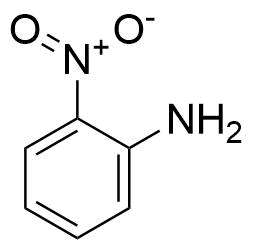
\includegraphics[width=0.2\textwidth]{pics/2-na.png}}
    \sidesubfloat[]{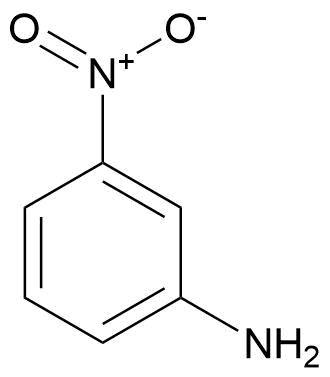
\includegraphics[width=0.2\textwidth]{pics/3-na.png}}
    \sidesubfloat[]{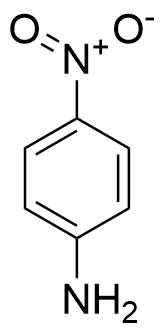
\includegraphics[width=0.125\textwidth]{pics/4-na.png}}
    \caption{Structure of (a) 2-nitroaniline, (b) 3-nitroaniline and (c) 4-nitroaniline.}
    \label{fig:na_structure}
\end{figure}




%\begin{figure}
%\vspace{0.5cm}
%  \sidesubfloat[]{\scalebox{0.7}{\begin{tikzpicture}\chemfig{**6(---(-[::-60]N(-[::60]H)-[::-60]H)-(-[::-60]N^{+}(=[::60]O)-[::-60]O^{-})--)}\end{tikzpicture}}\label{fig:nit1}}
%\qquad
%  \sidesubfloat[]{\scalebox{0.7}{\begin{tikzpicture}\chemfig{**6(--(-[::-60]N(-[::60]H)-[::-60]H)--(-[::-60]N^{+}(=[::60]O)-[::-60]O^{-})--)}\end{tikzpicture}}\label{fig:nit2}}
%\qquad
%  \sidesubfloat[]{\scalebox{0.7}{\begin{tikzpicture}\chemfig{**6(-(-[::-60]N(-[::60]H)-[::-60]H)---(-[::-60]N^{+}(=[::60]O)-[::-60]O^{-})--)}\end{tikzpicture}}\label{fig:nit3}}
  %\caption{Structure of (a) 2-nitroaniline, (b) 3-nitroaniline and (c) 4-nitroaniline.}\label{fig:nit}
%\end{figure}





\section{Experimental details}

\subsection{Selective Reagent Ion-Mass Spectrometry (SRI-MS)}
The SRI-MS instrument used was a KORE Technology Ltd PTR-ToF-MS, and 
the different reagent ions were generated injecting different gases into its ion source.
This device has been described in detail %in \autoref{chapter:ptr} and  
elsewhere \cite{RF_TNT,ellis2013proton}, so only a shallow overview will be given here.
%For this investigation, a KORE Technology Ltd. Series I Selective Reagent Ion-Time of Flight-Mass Spectrometer (SRI-ToF-MS) instrument was used, details of which been given elsewhere, \cite{ellis2013proton,blake2009proton} and therefore only brief and pertinent details will be presented in this paper. 

\subsubsection{Proton Transfer Reaction Mode}
This mode has been described in \autoref{chapter:ptr} and corresponds to the regular use of the instrument, where H$_3$O$^+$ (and the relevant water cluster ions) react with the analyte through the reactions described in \autoref{eq:pt} and \autoref{eq:ptc}. 
It is important to note, however, that, although proton transfer can be spontaneously dissociative, the energy available upon proton transfer from a protonated water cluster is much less than that compared to proton transfer from hydronium.
Nevertheless, the reduced electric field in the reactor can trigger collisional induced dissociation when the proton transfer process has been non-dissociative, enhancing fragmentation of the protonated molecule.
%This mode exploits the proton transfer reaction of H$_3$O$^+$ and, depending on the reduced electric field (the ratio of the electric field strength (E) to the gas number density (N)) applied in the drift tube and the humidity, also protonated water clusters with molecules of interest M: 

%\begin{equation}
%\label{eq:pa:nitro}
%    H_3O^+.(H_2O)_n + M \rightarrow MH^+ + (H_2O)_{n+1}   
%\end{equation}
%where n = 0, 1 and 2 are the most important for our operational conditions (see \autoref{fig:na_fig1}), but also (in low concentrations and only at low \textit{E/N} (less than approximately 100 Td (1 Td = 10$^{-17}$ V cm$^2$)) n = 3. Proton transfer can either be non-dissociative or spontaneously dissociative. Following non-dissociative proton transfer, collisional induced dissociation may occur, with the probability of this increasing with increasing reduced electric field.

\begin{figure}%[h]
\centering
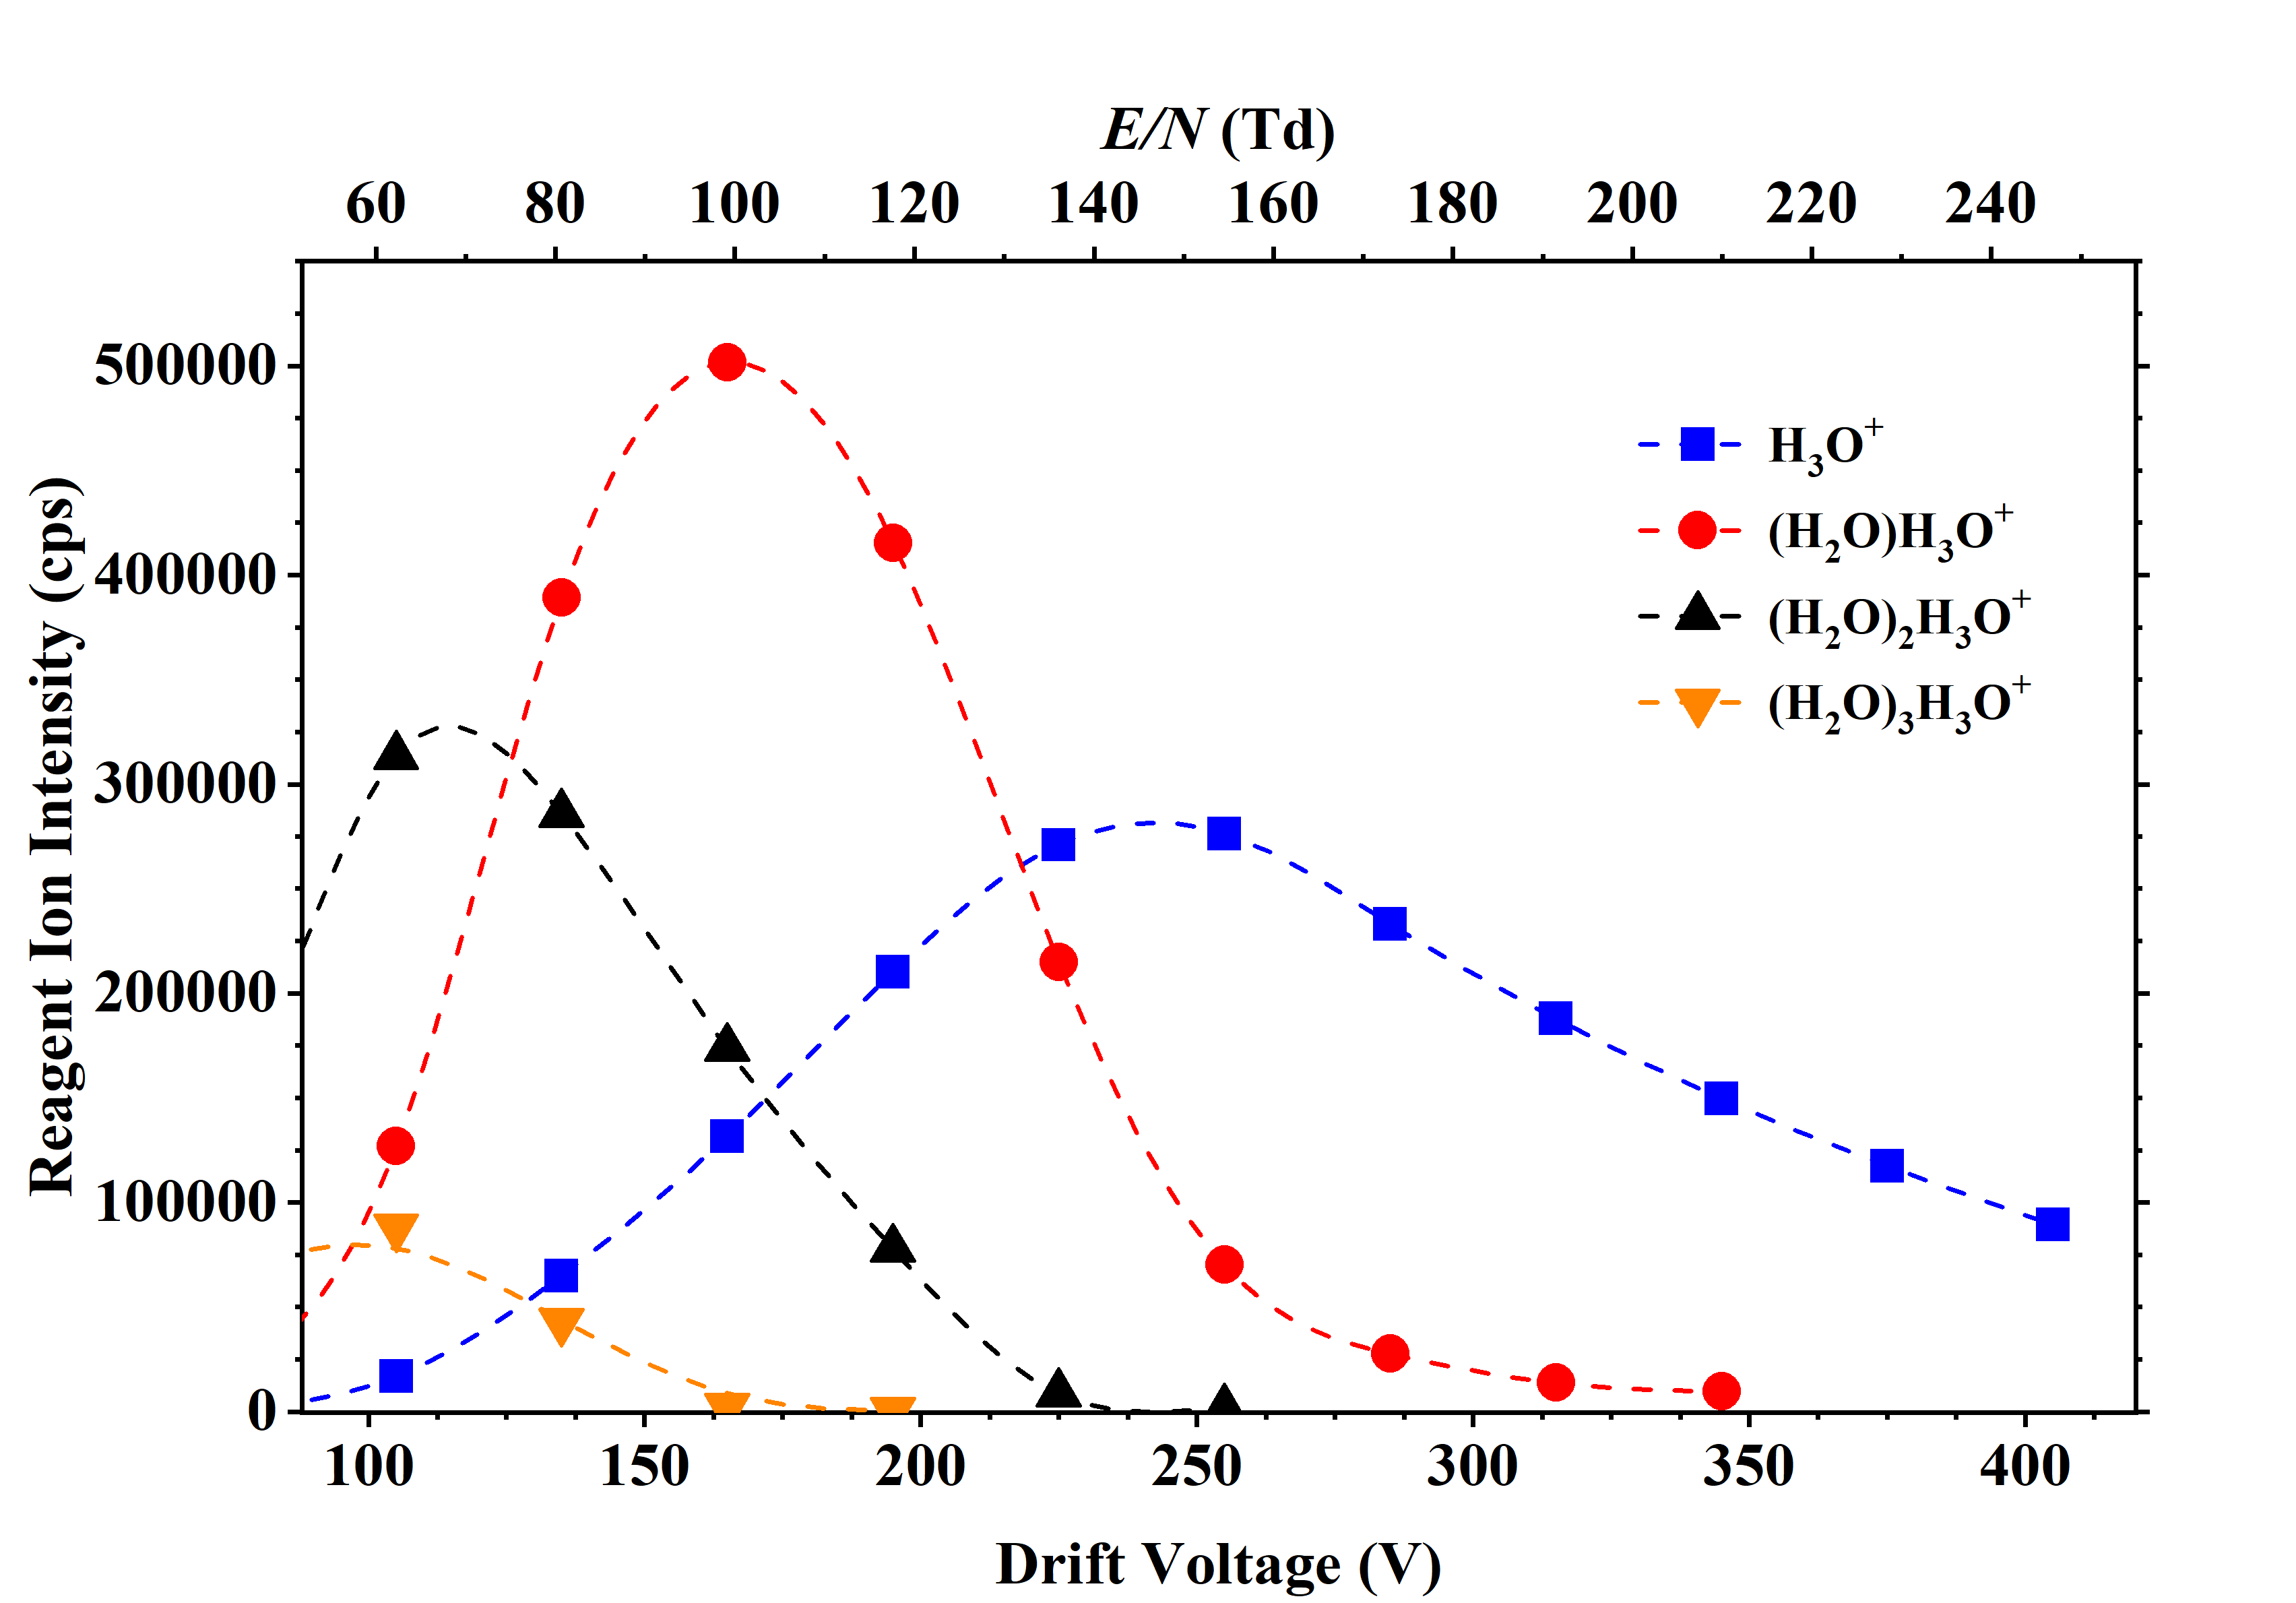
\includegraphics[height=0.35\textheight]{pics/nitros_paper_1.png}
\caption{Ion intensities in counts per second of the water reagent ions (H$_3$O$^+$.(H$_2$O)$_n$, n = 0, 1, 2 and 3) recorded at the detector of the KORE SRI-ToF-MS as a function of reduced electric field (approximately 60-250 Td).}
\label{fig:na_fig1}
\end{figure}

The reagent ions for proton transfer mode were produced through the injection of water into the hollow cathode. These are then transferred into the drift tube. 
\autoref{fig:na_fig1} presents the reagent ion intensities (in counts per second) at the end of the drift tube as a function of the \textit{E/N} and it shows that H$_3$O$^+$(H$_2$O)$_n$ for n = 0, 1 and 2 are the most abundant water clusters, although the one with n = 3 is also noticeable at low \textit{E/N}.
Only at \textit{E/N} values of 130 Td of more  H$_3$O$^+$ becomes the dominant ion. 
Other impurity or contamination ions can sometimes be observed in the mass spectra, resulting from the back streaming of the analyte-containing buffer gas into the hollow cathode. The most usual impurity ions are NO$^+$ and O$_2^+$, which, in this case, represented less than 0.5\% of the total reagent ion signal for any reduced electric field. 
Also, the signal corresponding to hydronium and the water cluster ions is usually saturated and the intensity at the $^{18}$O isotope was used in each case to calculate the signal of the relevant reagent ion.
%To produce the reagent ions, a series of ion/molecule processes (including three-body association) take place in a hollow cathode glow discharge, initiated by an electric discharge in water vapour and associated drift tube buffer gas that has diffused back into the ionisation source. The reagent ions that are generated in the ion source region are transferred into the drift tube by an applied voltage gradient. The relative intensities of the water reagent ions in the drift tube of the KORE instrument used as a function of \textit{E/N} are summarised in \autoref{fig:na_fig1}, which illustrates that under our operating conditions, only at relatively high \textit{E/N} values (greater than 140 Td) does H$_3$O$^+$ become the dominant reagent ion. 

%Although H$_3$O$^+$ (and associated protonated water clusters – depending on the value of the reduced electric field) dominates the reagent ion signal, other reagent ions are always present in the drift tube. These “impurity” reagent ions result from back diffusion of the buffer gas in the drift tube into the ion source. These reagent ions are those that cannot react with water, such as O$_2^+$. However, these are at very low concentrations. Under our experimental conditions, the intensity of O$_2^+$ was maintained below 0.5\% of that of the H$_3$O$^+$ signal.

%The signal intensity of H$_3\,^{16}$O$^+$ is generally too large to be measured directly. Therefore, the signal intensity for the spectral line peaking at \textit{m/z} 21.02, corresponding to H$_3\,^{18}$O$^+$, was recorded. The \textit{m/z} 19.02 intensity, corresponding to H$_3\,^{16}$O$^+$, was determined in the normal manner by multiplying the \textit{m/z} 21.02 signal by 487. Similarly, the \textit{m/z} 37.03 signal intensity, corresponding to H$_3\,^{16}$O$^+$·H$_2\,^{16}$O, was not measured directly. Instead the signal intensity at \textit{m/z} 39.03 (H$_3\,^{18}$O$^+$.H$_2\,^{16}$O or H$_3\,^{16}$O$^+$.H$_2\,^{18}$O) was recorded and multiplied by 243. 


\subsubsection{Charge Transfer Reaction Mode}
O$_2^+$ was generated injecting pure oxygen (99.998\% purity, BOC Gases, Manchester, UK) into the hollow cathode.  
The O$_2^+$ ion signal as a function of the reduced electric field is displayed in \autoref{fig:na_fig2}.    
Similarly to the reagent ion in the proton transfer mode, the O$_2^+$ signal is too large to be directly measured and the $^{18}$O$^{16}$O$^+$ isotope at \textit{m/z} 34 can be used to calculate it.
When O$_2^+$ encounters the analyte in the drift tube, charge transfer occurs if the analyte's ionisation energy (\acrshort{ie}) is less than 12.07 eV.
However, and contrary to what happens in proton transfer, even if the analyte has an ionisation energy of less than 12.07 eV, the reaction may not be occuring at the collisional rate  \cite{jarvis2000charge}. 
Like in proton transfer, charge transfer can be either non-dissociative, yielding the M$^+$ ion, or dissociative, and fragmentation can be enhanced upon collisionally-induced proccesses. 
Regarding contamination and unwanted ions, hydronium can be formed in the ion source if there is residual water vapour but in these experiments it was only ca. 0.1\% of the O$_2^+$ signal.

%For the production of O$_2^+$, pure oxygen (99.998\% purity, BOC Gases, Manchester, UK) was flowed into the ion source. This leads to the formation of mainly O$_2^+$ reagent ions (> 95\%). \autoref{fig:na_fig2} shows the O$_2^+$ ion signal intensity in counts per second (cps) as a function of E/N. Once injected into the drift tube, O$_2^+$ may react with the analyte M via charge transfer, provided that the ionisation energy (IE) of M is less than that of O$_2$ (IE (O$_2$) = 12.07 eV). Unlike proton transfer, an exothermic reaction is a necessary but not sufficient criterion for charge transfer to occur, and hence the reaction rate coefficient may not necessarily be collisional \cite{jarvis2000charge}. However, if charge transfer does occur, it may also be either non-dissociative (resulting in the singly charged parent ion, M$^+$) and/or dissociative. Fragmentation might be spontaneous upon charge transfer or require additional energy through collisions in the drift tube. H$_3$O$^+$ is also observed when operating the ion source in oxygen mode. This is due to residual water vapour in the system. However, this can be ignored owing to its signal intensity being approximately 0.1\% of the O$_2^+$ signal for the experimental conditions used throughout our measurements.

\begin{figure}%[h]
\centering
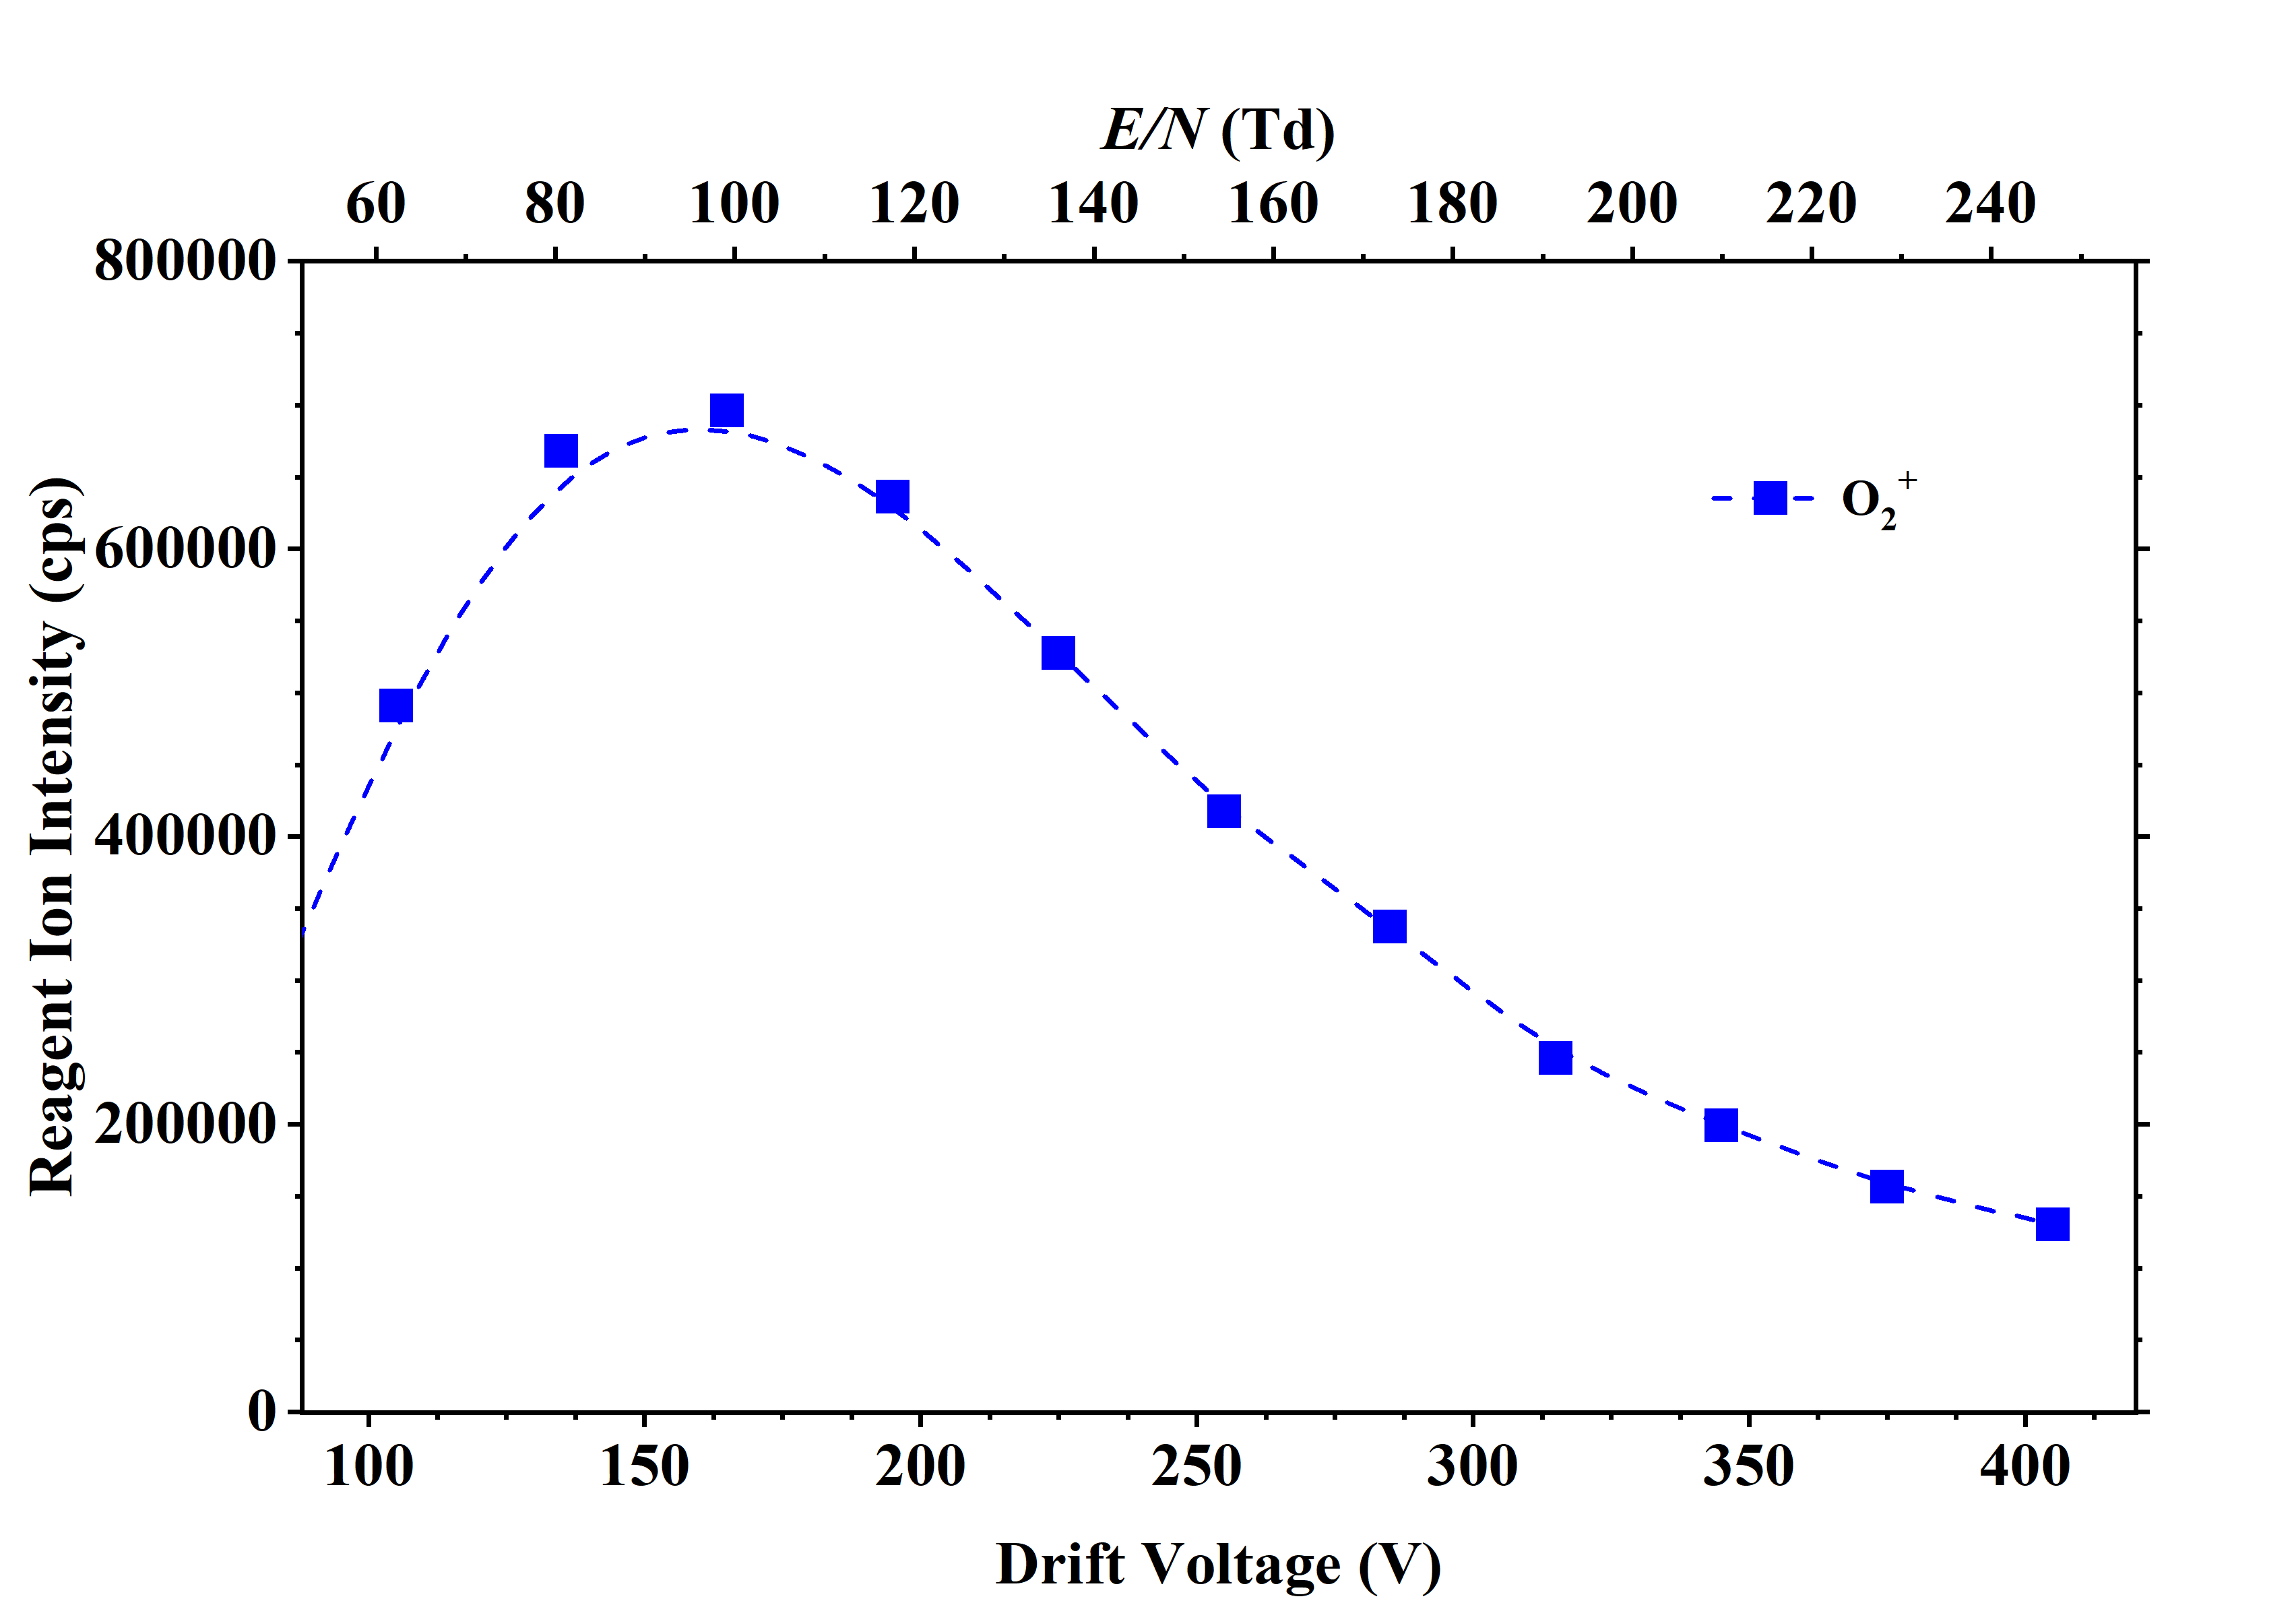
\includegraphics[height=0.35\textheight]{pics/nitros_paper_2.png}
\caption{Ion intensities in counts per second of O$_2^+$ recorded at the detector of the KORE SRI-ToF-MS as a function of reduced electric field (approximately 60-250 Td).}
\label{fig:na_fig2}
\end{figure}

\subsection{Chemicals}
The samples in this investigation were acquired from Sigma Aldrich (Cheshire, UK). Each of the three nitroaniline isomers (yellow granulated solids, >98\% purity) came in an individual container. 
Each of these substances were then used to create a solution of approximately 100 µg/mL of concentration in a mixture of methanol and acetonitrile (analytical grade).
1 µL of this diluted sample was placed on a swab, waiting one minute for the solvent to evaporate before inserting it into the TDU.
The vapour pressure of 2-, 3- and 4- nitroaniline is 3.7$\times$10$^{-3}$, 1.3$\times$10$^{-4}$, and 4.3$\times$10$^{-6}$ mbar, respectively \cite{2na,3na,4na}.
%Individual nitroaniline (2-, 3- and 4-) isomers for this study were purchased from Sigma Aldrich (Cheshire, UK), all of which came with stated purities of at least 98\%. At room temperature, nitroanilines are yellowish-orange granulated solids. For the measurements, granules were dissolved in a mixture of MeOH:AcN 1:1 (V/V) (analytical grade) to provide a concentration of approx. 100 µg/mL. A volume of 1 µL of this solution was deposited onto the swab and left the solvents to evaporate at room temperature for approximately one minute before placing the swab into the TDU.




\subsection{Operational procedures}
The thermal desorption unit, described in \autoref{section:tdu} and also elsewhere \cite{RN445}, was used in this study to get the nitroanilines solution into gas phase. Said TDU was connected to the inlet line through passivated Silconert\textsuperscript{\textregistered} stainless steel and the carrier gas flowing through the TDU was oxygen-free nitrogen (99.998\% purity, BOC Gases, Manchester, UK). 
Three measurements were acquired for each \textit{E/N} value, which were then averaged and got the background subtracted. 
The reactor, inlet line and thermal desorption unit were kept at 150$^{\circ}$C. The drift tube was at 1 mbar and the ion source at 1.4 mbar when generating both H$_3$O$^+$ and O$_2^+$.
The reduced electric field was manipulated only by adjusting the drift voltage in the reactor in the range from approximately 100 to 400 V, which corresponds to a \textit{E/N} range from approximately 60 to 250 Td.
%Liquid samples were vaporised making use of a thermal desorption unit (TDU), connected to the inlet of the drift tube via passivated stainless steel (Silconert\textsuperscript{\textregistered}). Details of the TDU have been given elsewhere \cite{RN445}. The TDU, connecting lines and drift tube were operated at a temperature of 150$^{\circ}$C. For this study oxygen-free nitrogen (99.998\% purity, BOC Gases, Manchester, UK) was used as the carrier gas. PTFE swabs (ThermoFisher Scientific, Cheshire, UK), onto which known quantities of the sample had been deposited, were manually placed into the TDU. Upon closure of the TDU unit a high force annular “anvil” compressed the PTFE to plastically deform and convert it into a gas tight circular seal around the rim of the swab. At the same time laboratory air heated to a specified temperature rapidly heats the PTFE and as it passes through carries any thermally desorbed material into the heated inlet line through to the drift (reaction) region. The temporal desorption profile is typically between 10-20 seconds \cite{RN445}. For each measurement one swab was used, which was replicated three times. The results were then averaged and any background signals were subtracted. 

%The drift tube pressure was set at 1 mbar and the glow discharge (for both water vapour and oxygen) was set at 1.4 mbar. The only variable was the operating drift tube voltage, which was adjusted over a range of approximately 100 to 400 V to provide an appropriate reduced electric field range of about 60-250 Td. 


\subsection{Density Functional Theory Calculations}
The proton affinities and gas-phase basicities of the three nitroaniline isomers and the water monomer, dimer and trimer were computed through DFT calculations using Gaussian09W and GaussView05 for Windows by Dr Peter Watts \cite{frisch2009gaussian}. 
The functional and the basis set used for this calculations were the B3LYP and 6-31+G(d,p), respectively, which have proved adequate in past studies \cite{GonzalezMendez2017939,gonzalez2017ion}.
%Density functional theory (DFT) calculations have been undertaken to determine the proton affinities and gas-phase basicities of the water monomer, dimer and trimer and the three nitroanilines. These calculations were conducted using Gaussian09W and GaussView05 for Windows \cite{frisch2009gaussian}. The B3LYP functional with the 6-31+G(d,p) basis set was used throughout, a combination which has been found to be satisfactory based on our previous work \cite{GonzalezMendez2017939,gonzalez2017ion}.


\section{Results}
In this section the experimental and DFT results are presented. 
The experimental work consists on the product ion distributions (PID) resulting from the reaction of each nitroaniline isomer with the proper reagent ion as a function of the reduced electric field (top x-axis) and the drift voltage (bottom x-axis).
All the isotopologues were taken into account when calculating the product ion distributions, although only the lightest one is given.
The uncertainty has been estimated to be around 10\% for any of the percentages provided here.% and only product ions representing more than 1\% of the total product ion signal were reported.
%For this section only product ions with branching percentages greater than 1\% for any given reduced electric field value are reported. The uncertainty in any branching percentage is approximately 10\%. In all cases only the mass to charge ratio of the lightest isotope is given. However, when calculating the product ion distributions we considered all of the isotopologues. For the product ion distribution (PID) plots (branching percentages) the voltage applied to the drift tube is shown in the main x-axis, and the reduced electric field \textit{E/N} achieved for that particular voltage is showed in the secondary x-axis.


\subsection{DFT Results}
The proton affinity and gas-phase basicity for the nitroaniline isomers and the water monomer, dimer and trimer are shown in \autoref{table:nitros}, which also includes the ionisation energies of O$_2$ and the nitroanilines \cite{linstrom2015nist}. 
Furthermore, \autoref{table:nitros} also contains the calculations for the change in the enthalpy, $\Delta$H$_{298}$,  and Gibbs free energy, $\Delta$G$_{298}$, for the addition of H$_2$O to the already protonated nitroaniline molecule.
The calculated thermochemical data related to the proton transfer case (i.e. PA, GB, $\Delta$H$_{298}$ and $\Delta$G$_{298}$) is given independently for the amino and nitro groups for comparison. 
These quantities were also calculated for the aniline and nitrobenzene molecules.
%\autoref{table:nitros} presents the calculated proton affinities and gas phase basicities for the water monomer, the water dimer, the water trimer and the three nitroanilines. For the nitroaniline isomers, values are provided for the two possible protonation sites, namely on the amino and nitro groups. Aniline and nitrobenzene are also shown for comparison. \autoref{table:nitros} also provides for convenience the ionisation energies of oxygen and the nitroanilines \cite{linstrom2015nist}.



\begin{table}[t]
\caption{Proton affinities, gas phase basicities and ionisation energies for nitroaniline isomers. The PA and GB values have been calculated using the B3LYP functional and the 6-31+G(d,p) basis set at 298 K. $\Delta$H$_{298}$ and $\Delta$G$_{298}$ refer to the enthalpies and free energies for the addition of water to the protonated species. For convenience the ionisation energies of O$_2$ and the three nitroanilines are also provided.}
\label{table:nitros}
\begin{tabular}{lcccccc}
\hline
\textbf{Chemical}              & \textbf{Site} & \textbf{PA\footnotemark} & \textbf{GB\footnotemark[\value{footnote}]} & \textbf{$\Delta$H$_{298}$\footnotemark[\value{footnote}]} & \textbf{$\Delta$G$_{298}$\footnotemark[\value{footnote}]} & \textbf{IE\footnotemark }             \\
\hline
Water                 &      & 684 & 653 &     &     &                       \\
\hline
Water dimer           &      & 842 & 777 &     &     &                       \\
\hline
Water trimer          &      & 937 & 841 &     &     &                       \\
\hline
O$_2$                    &      &     &     &     &     & 12.07 \cite{tonkyn1989rotationally}               \\
\hline
\multirow{2}{*}{2-NA} & NH$_2$  & 840 & 806 & -69 & -37 & \multirow{2}{*}{8.27} \\
\cline{2-6}
                      & NO$_2$  & 858 & 824 & -76 & -43 &                       \\
\hline
\multirow{2}{*}{3-NA} & NH$_2$  & 824 & 796 & -78 & -43 & \multirow{2}{*}{8.31} \\
\cline{2-6}
                      & NO$_2$  & 830 & 800 & -84 & -51 &                       \\
\hline
\multirow{2}{*}{4-NA} & NH$_2$  & 810 & 784 & -78 & -43 & \multirow{2}{*}{8.34} \\
\cline{2-6}
                      & NO$_2$  & 879 & 847 & -73 & -39 &                       \\
\hline
Aniline               & NH$_2$  & 874 & 846 & -72 & -40 &                       \\
\hline
Nitrobenzene          & NO$_2$  & 806 & 775 & -90 & -55 &                      \\
\hline
\addtocounter{footnote}{-1}
\footnotetext{\footnotemark[\value{footnote}]Thermochemical data expressed in kJ/mol.\addtocounter{footnote}{1}
\footnotemark[\value{footnote}]Ionisation energies (in eV) have been taken from NIST database \cite{linstrom2015nist}.} 
\end{tabular}
\end{table}


It is interesting to note that the PA and GB of the amine group in the  aniline molecule are higher than those of the nitro group in nitrobenzene, but when both functional groups are present in the same molecule (i.e. for the three nitroaniline isomers), the values of PA and GB of the amine and nitro groups are reversed.%smaller than those of the nitro group.
This is caused by the NH$_2$ group donating electrons to the benzene ring and the NO$_2$ group pulling electrons from said ring. 
The calculated basicities show that all three nitroanilines can undergo proton transfer from H$_3$O$^+$ and H$_3$O$^+$.(H$_2$O), and that 4-nitroaniline can also do it from H$_3$O$^+$.(H$_2$O)$_2$ to its nitro group.
As proton transfer to both groups of the nitroanilines is exoergic, NA.H$^+$ is thought to be a mixture of parent molecules protonated at the NH$_2$ and the NO$_2$ sites. However, as in 2-nitroaniline the two functional groups are very close, there the proton sits bonded to both functional groups.
%As shown in \autoref{table:nitros}, whilst for simpler chemical structures as aniline and nitrobenzene, the aniline’s NH$_2$ substituent is much more basic than the NO$_2$ of nitrobenzene, this is not the case in the nitroanilines where both groups are on the ring. The interaction of the nitro group (electron withdrawing effect from the aromatic ring) and the amine group (electron donating effect to the aromatic ring) reverse their basicities, in the order 4-NA > 2-NA > 3-NA. Based on this data, with the exception of the 2-NA where the groups are in close proximity it is likely that the NA.H$^+$ for the 3 and 4 isomers is a mixture of species. The DFT calculations show that proton transfer from H$_3$O$^+$.(H$_2$O)$_n$ (n = 0 and 1) to both sites of all three of the nitroanilines is exoergic. H$_3$O$^+$.(H$_2$O)$_2$ can also proton transfer to the NO$_2$ site of 4-NA.





\subsection{Fragmentation patterns and branching ratios studies in proton transfer mode}

\subsubsection{2-nitroaniline}
The product ion distributions for the reaction of 2-nitroaniline with H$_3$O$^+$ and H$_3$O$^+$.(H$_2$O) from 60 to 250 Td is shown in \autoref{fig:na_fig3}. 
The most abundant ion from 60 to ca. 230 Td is the protonated parent molecule 2-NA.H$^+$ at \textit{m/z} 139.05.
The ion coming from the association of the protonated parent with a water molecule (i.e. 2-NAH$^+$.H$_2$O at \textit{m/z} 157.06) is present at low \textit{E/N}, and it decreases with the increasing \textit{E/N}, with a maximum contribution to the total ion signal of $\sim$15\% at 60 Td.
Additionally, further product ions are observed at high reduced electric fields. 
C$_6$H$_5$N$_2$O$^+$ at \textit{m/z} 121.04, which comes from the loss of water from the protonated parent, appears at 150 Td and becomes dominant at approximately 230 Td.
Likewise, C$_6$H$_7$N$^+$ at \textit{m/z} 93.06 and C$_6$H$_5$N$^+$ \textit{m/z} 91.04 are also observed at high \textit{E/N}. 
The former results from the loss of a nitro group from 2-NA.H$^+$, while the latter comes from the loss of a hydrogen molecule after a loss of a nitro group from the protonated parent.

The mass spectra shown in \autoref{fig:na_spec} are included as illustrative examples of the data acquired when performing these experiments. 
These two different data sets relate to measurements of 2-nitroaniline with different \textit{E/N} values in the drift tube, while the rest of variables were kept constant. 
Comparable mass spectra were found with the rest of compounds in both proton transfer and charge transfer modes, but these are not included as those results are summarised in the PID plots, which include the product ions with a branching percentage higher than >1\% for any \textit{E/N}.

%\autoref{fig:na_fig3} shows the product ion distribution plot for 2-nitroaniline resulting reactions with H$_3$O$^+$.(H$_2$O)$_n$ (n = 0 and 1) (see \autoref{fig:na_fig1}) as a function of \textit{E/N} over the range from 60 to 250 Td. The protonated parent, [2-NA.H]$^+$at \textit{m/z} 139.05 is the most intense product ion until about 220 Td, after which fragment product ions dominate. Fragment product ions begin to appear at about 150 Td, starting with at \textit{m/z} 121.04 (resulting from the loss of a water molecule from the protonated parent, [2-NA - H$_2$O]H$^+$), and which becomes dominant above about 220 Td. Other fragment product ions are observed with increasing E/N, namely \textit{m/z} 93.06 (assigned to the loss of a nitro group from the protonated parent, leading to a C$_6$H$_7$N$^+$ ion) and \textit{m/z} 91.04 (caused by the loss of a nitro group followed by the sequential loss of a hydrogen molecule, leading to a C$_6$H$_5$N$^+$ ion). At low reduced electric fields (less than about 120 Td) a product ion is observed at \textit{m/z} 157.06, which is simply 2-NAH$^+$.H$_2$O, resulting from a third body association reaction of the protonated parent with water. Its intensity increases as the \textit{E/N} decreases because of reduced collisional induced dissociation.

%\autoref{fig:na_spec} shows two overlaid mass spectra at two different \textit{E/N} values for 2-nitroaniline, exemplifying the difference in performance for the instrument. Similar plots (not shown) were found for the rest of the samples and for oxygen chemistry. 

\begin{figure}%[h]
\centering
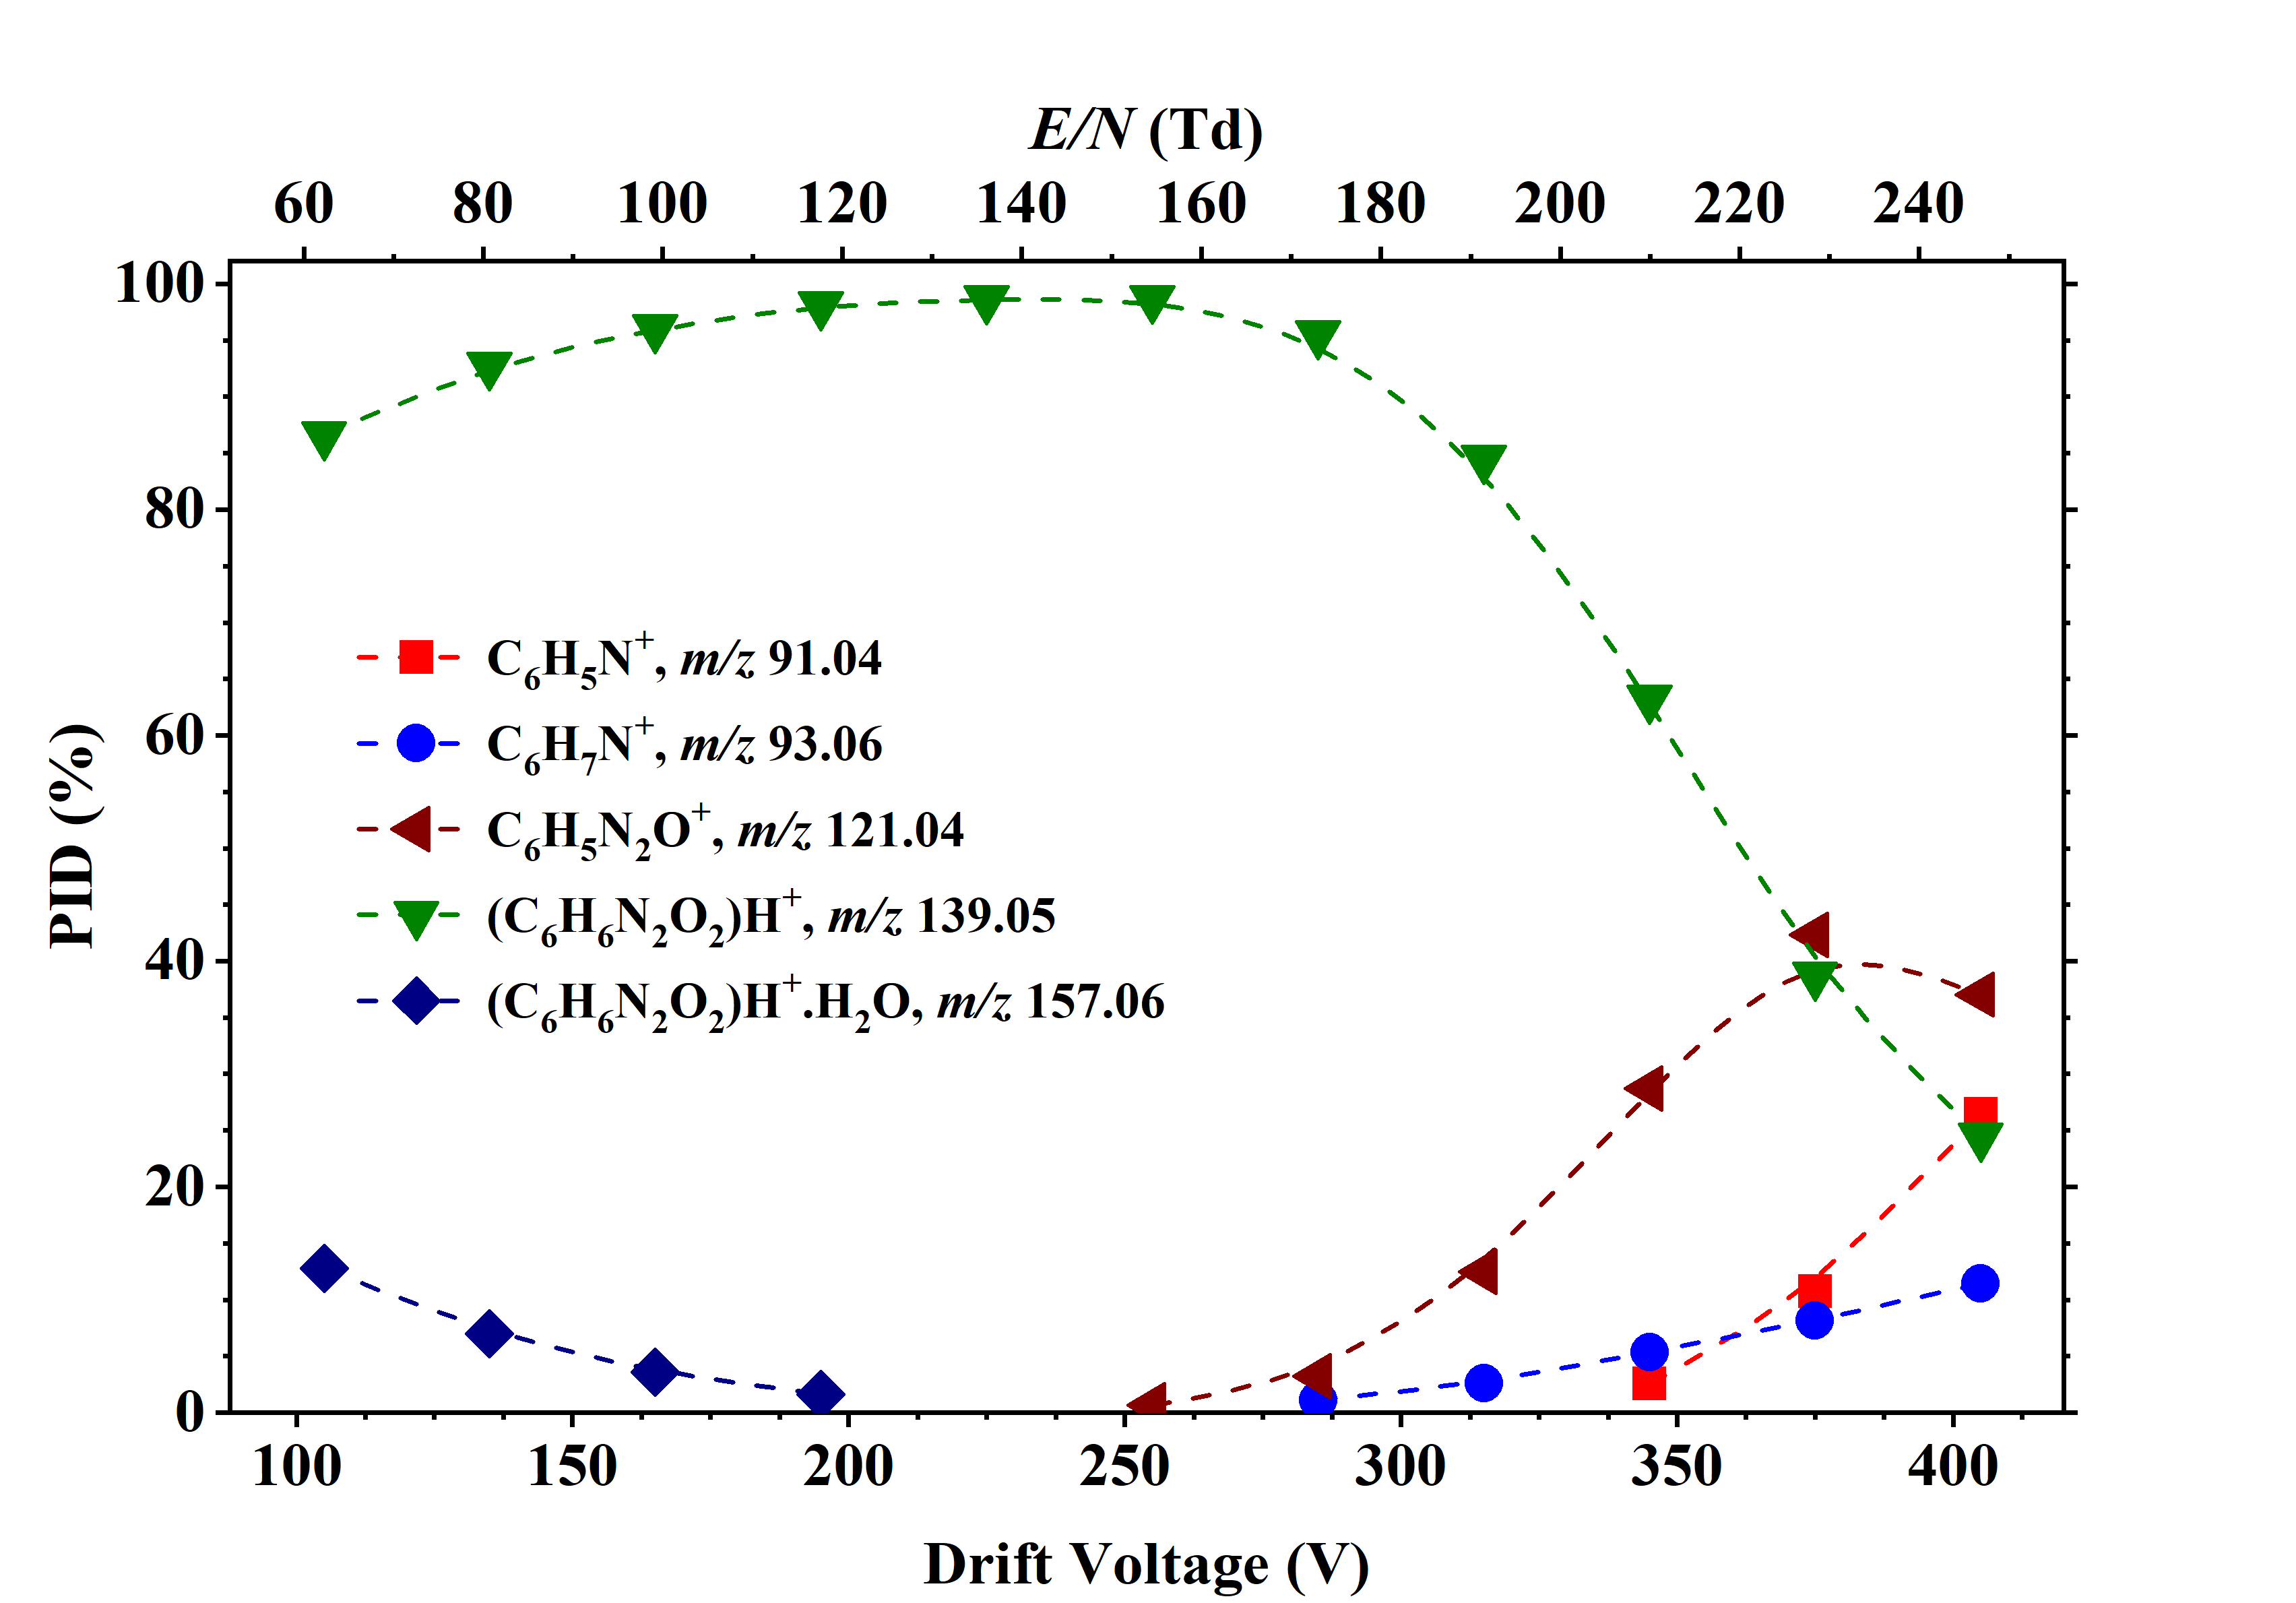
\includegraphics[height=0.35\textheight]{pics/nitros_paper_3.png}
\caption{Percentage product ion distribution (PID in \%) resulting from the reaction of 2-nitroaniline with H$_3$O$^+$.(H$_2$O)$_n$ (n = 0 and 1) as a function of the reduced electric field from 60 to 250 Td.}
\label{fig:na_fig3}
\end{figure}




\begin{figure}%[h]
\centering
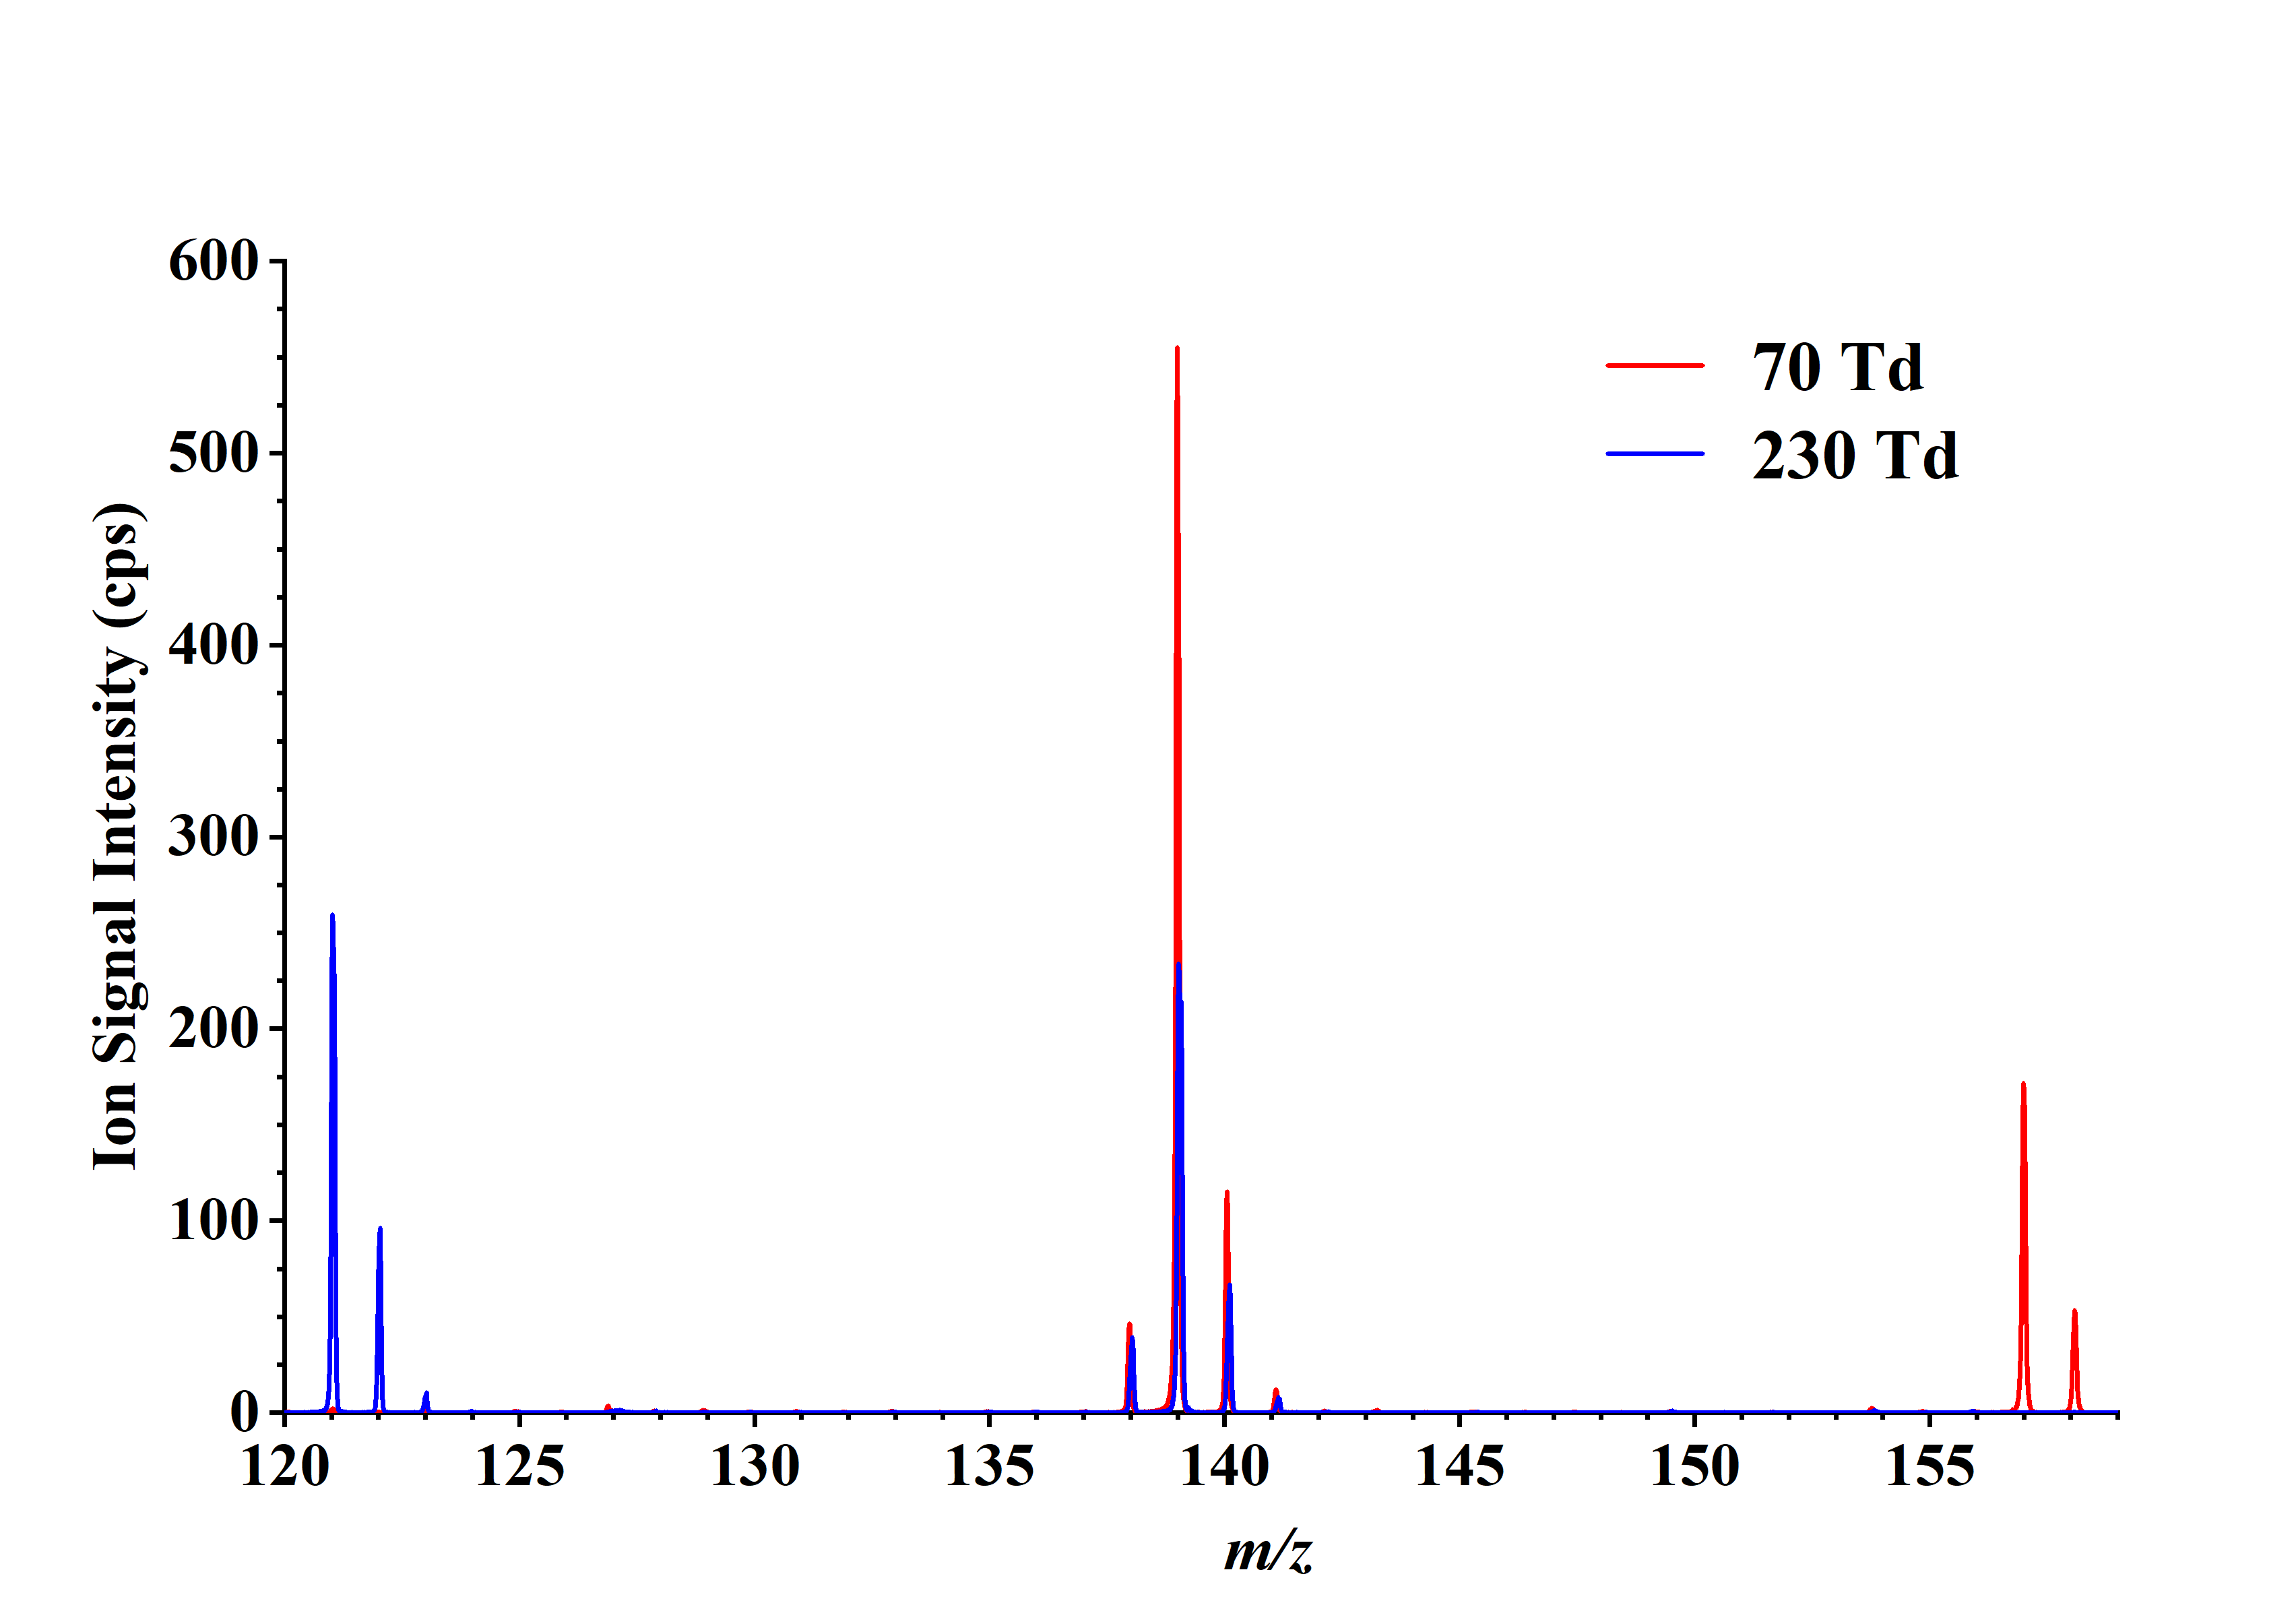
\includegraphics[height=0.35\textheight]{pics/nitros_paper_spec.png}
\caption{Overlaid mass spectra for 2-nitroaniline at 70 and 230 Td. This figure illustrates the clear difference in ion signal intensities for \textit{m/z} 121.04, 139.05 and 157.06 upon the reduced electric field applied to the DT of the instrument.}
\label{fig:na_spec}
\end{figure}


\subsubsection{3-nitroaniline}
The PID plot for the reaction of the 3- isomer with H$_3$O$^+$ and H$_3$O$^+$.(H$_2$O) (\autoref{fig:na_fig4}) shows that, like in the 2-NA case, the most abundant ion is the protonated parent, 3-NA.H$^+$ at \textit{m/z} 139.05, over a large reduced electric field range.
In addition to that, the three body association with water yielding 3-NA.H$^+$.H$_2$O is observed at low \textit{E/N}, but in the case of 3-nitroaniline the presence of this ion is much higher than that in the 2-nitroaniline experiment, reaching roughly 50\% at 60 Td and having the same intensity as the protonated parent signal.

On the other side, two other product ions are observed at high reduced electric field.
C$_6$H$_7$N$^+$ at \textit{m/z} 93.03 becomes the most abundant ion at around 230 Td.
At the same, C$_6$H$_7$NO$^+$ at \textit{m/z} 109.05, which was not found for 2-nitroaniline and comes from the loss of NO from the protonated parent, is observed for \textit{E/N} values higher than 190 Td.

%\autoref{fig:na_fig4} shows the PID plot for 3-nitroaniline resulting from its reaction with H$_3$O$^+$.(H$_2$O)$_n$ (n = 0 and 1) as a function of the reduced electric field \textit{E/N} for the range from 20 to 250 Td. Similar to the results obtained for 2-NA, the protonated parent [3-NA.H]$^+$is the dominant product ion up to about 220 Td. However, unlike 2-NA, much more association of the protonated parent with water is observed at low reduced electric fields (< 140 Td), under identical operational (reduced electric field and humidity) conditions. At 60 Td 3-NAH$^+$.H$_2$O has approximately the same branching percentage as the protonated parent. 

%Above ca. 230 Td the fragment product ion C$_6$H$_7$N$^+$ dominates. Another product ion, starting at an \textit{E/N} value of approximately 190 Td, is observed at \textit{m/z} 109.05. This is considered to result from the loss of NO from the protonated parent leading to C$_6$H$_7$NO$^+$ \cite{beynon1959some}. This product ion was not observed for 2-nitroaniline.

\begin{figure}%[h]
\centering
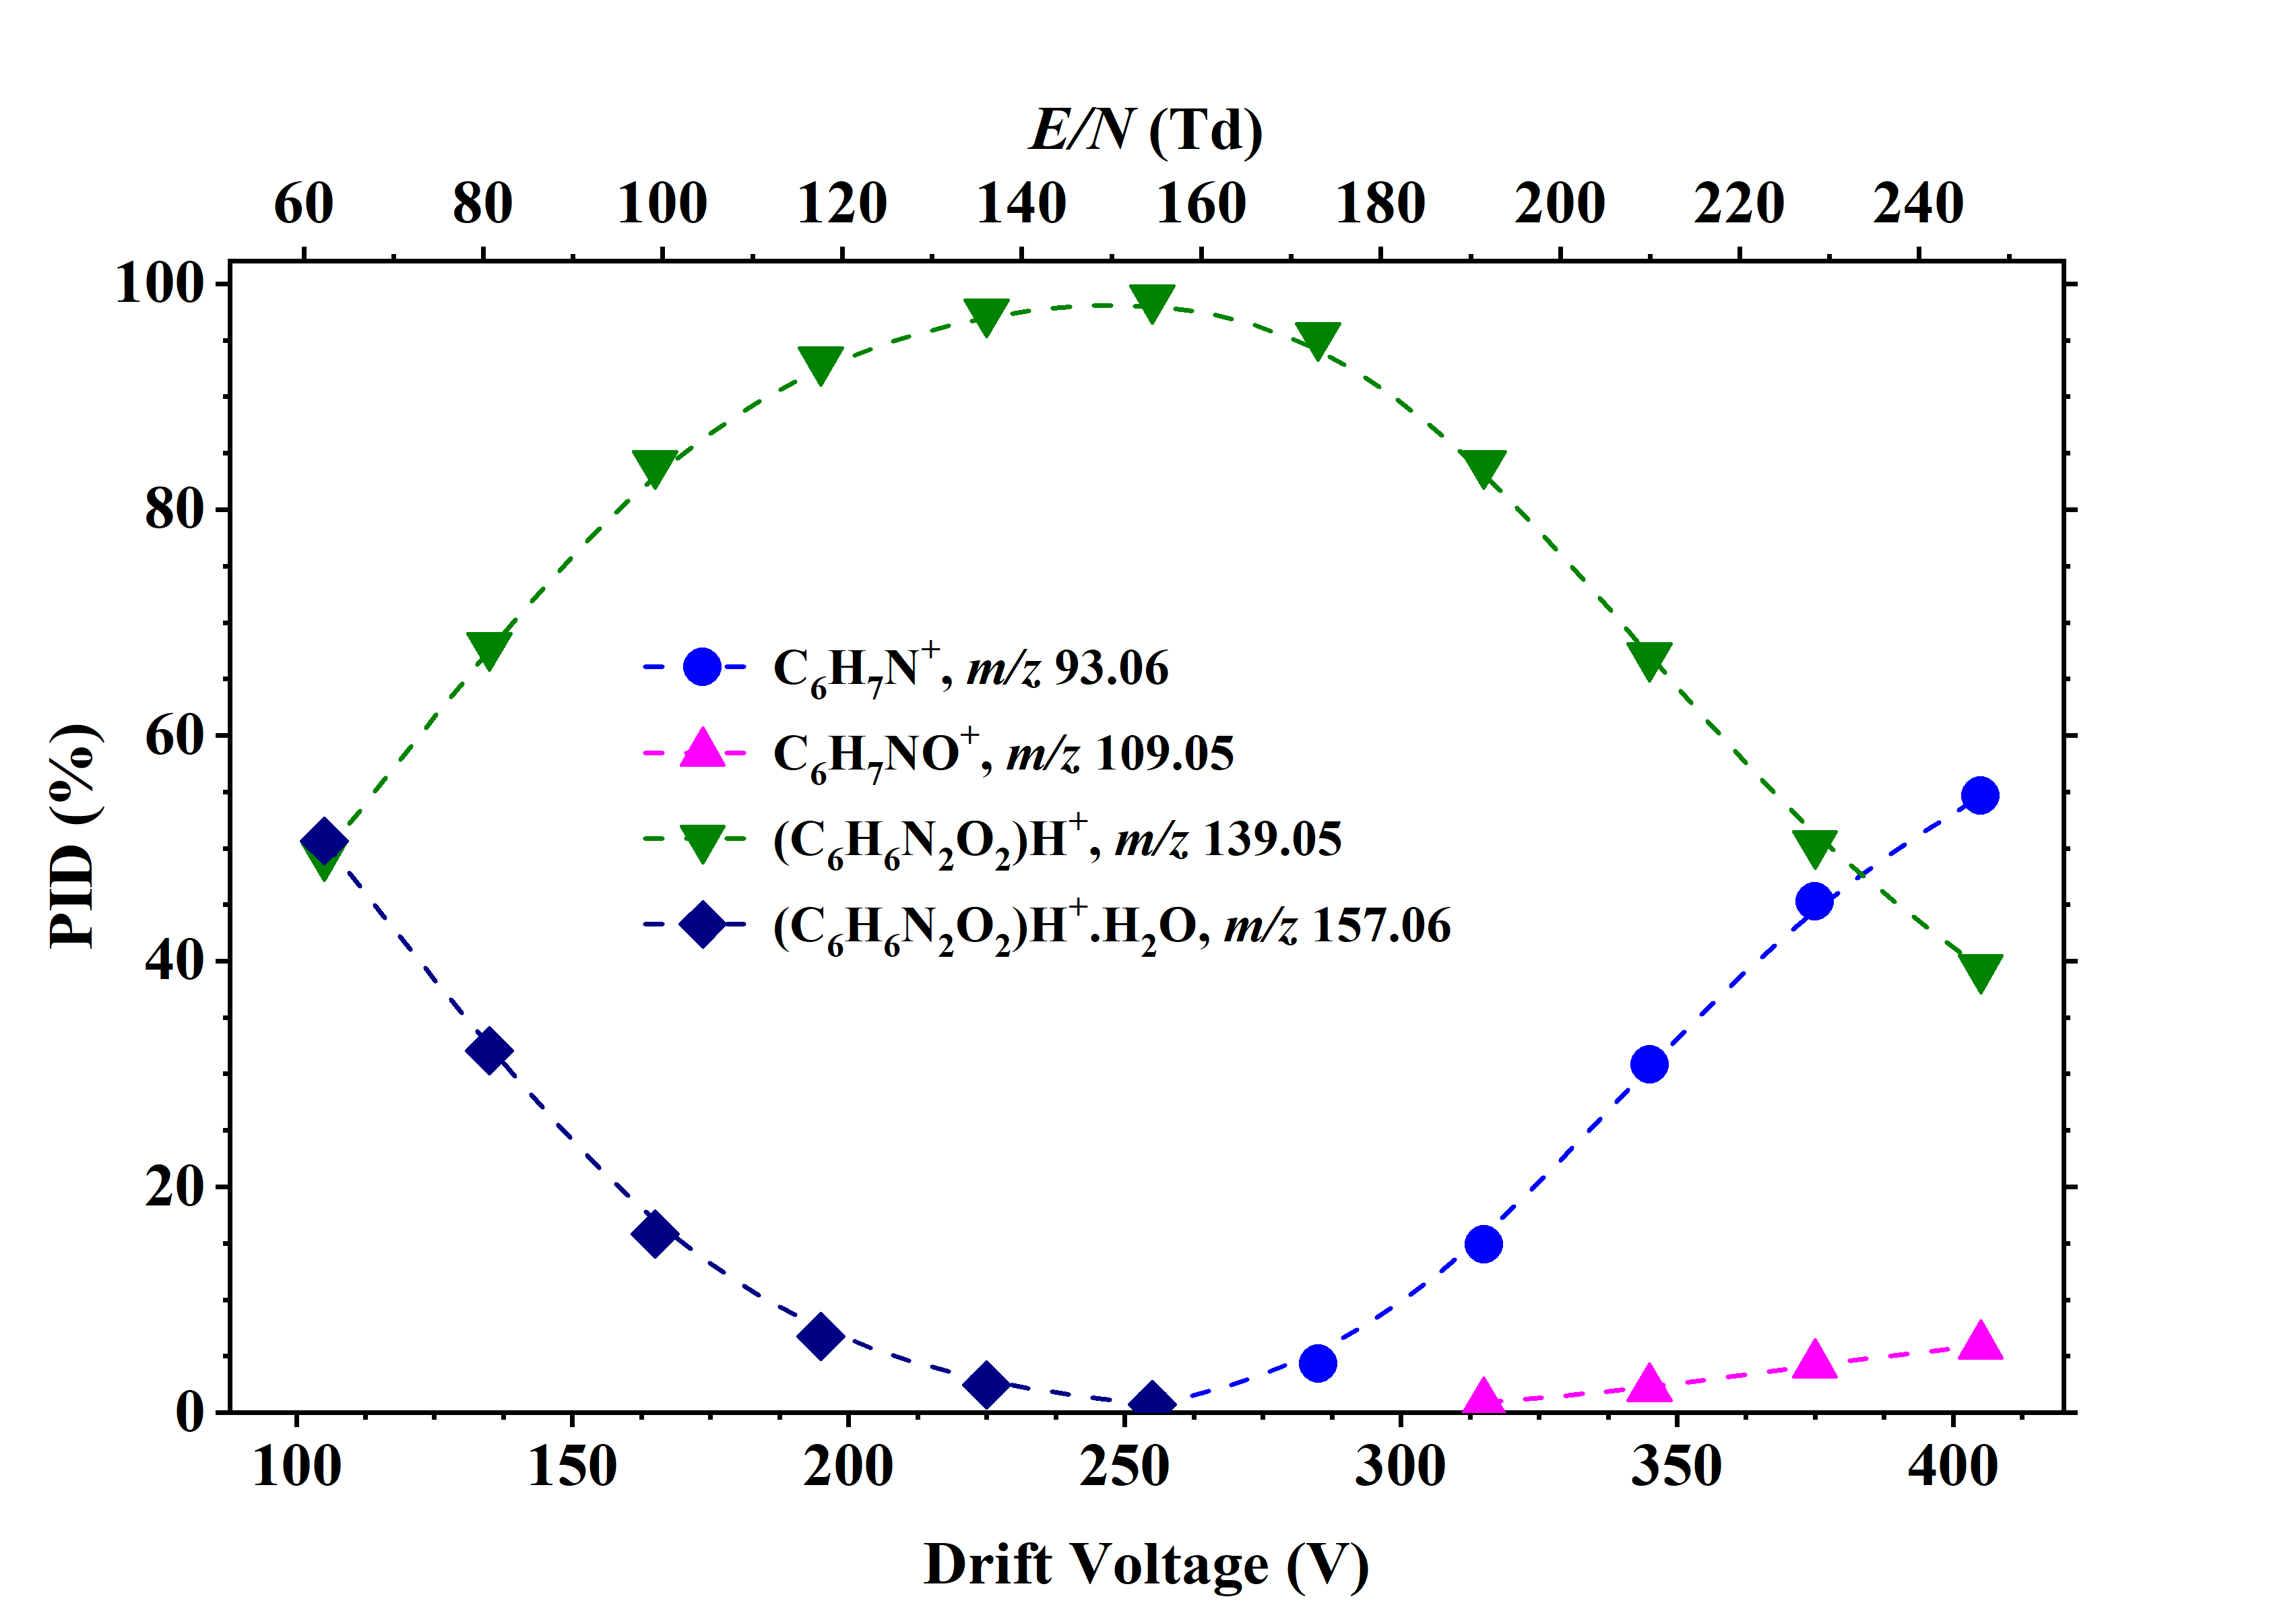
\includegraphics[height=0.35\textheight]{pics/nitros_paper_4.png}
\caption{Percentage product ion distribution resulting from the reaction of 3-nitroaniline with H$_3$O$^+$.(H$_2$O)$_n$ (n = 0 and 1) as a function of the reduced electric field from 60 to 250 Td.}
\label{fig:na_fig4}
\end{figure}

\subsubsection{4-nitroaniline}
The PID for the reaction of 4-nitroaniline with H$_3$O$^+$, H$_3$O$^+$.(H$_2$O) and potentially H$_3$O$^+$.(H$_2$O)$_2$ is shown in \autoref{fig:na_fig5}. 
The protonated parent (4-NA.H$^+$ at \textit{m/z} 139.05) is the most abundant ion across the whole reduced electric field range (>80\%).
The clustering with water at low \textit{E/N} has an intensity comparable to that in the 2-NA case (max 5-10\% at 60 Td) and the only fragment ion (C$_6$H$_7$N$^+$ at \textit{m/z} 93.06) is found at >160 Td.

A key result of these experiments is that protonated 3-nitroaniline shows more clustering with water than the other two isomers but this can be explained in terms of the thermochemical data presented in \autoref{table:nitros}.
The calculated change in the Gibbs free energy, $\Delta$G$_{298}$, for the clustering of 2-NA and 4-NA with water is 43 kJ mol$^{-1}$, while this is 51 kJ mol$^{-1}$ for 3-NA. 
This 8 kJ mol$^{-1}$ difference, translated into equilibrium constants  at 298 K (i.e. $exp(-\Delta G_{298}/RT)$), indicates that the solvation reaction is 25 times more effective for 3-NA.H$^+$ than for the other isomers. 
Furthermore, at the temperature of the drift tube (i.e. 150$^\circ$C, 423 K) 8 kJ mol$^{-1}$ represents a tenfold difference for the association of water with  3-NA.H$^+$ than for that with 2-NA.H$^+$ and 4-NA.H$^+$.


In the 4-nitroaniline molecule, the nitro and amine functional groups are in opposite sites of the aromatic ring, which makes it difficult to create a transition state between said functional groups which would result in further product ions. 
The main consequence of this feature is that, as mentioned above, the protonated parent is the largely dominant ion, showing less fragmentation than the 2- and 3- isomers, which is in agreement with the chemical ionisation results for mononitroarenes with electron-releasing substituents \cite{harrison1980chemical}.
%\autoref{fig:na_fig5} presents the PID for the reaction of 4-nitroaniline with H$_3$O$^+$.(H$_2$O)$_n$ (n = 0 and 1) as a function of the reduced electric field \textit{E/N} for the range from 60 to 250 Td. For this isomer, the protonated parent, [4-NA.H]+, dominates throughout the whole \textit{E/N} range. Little fragmentation occurs, with only one product ion being observed at \textit{m/z} 93.06 (corresponding to the loss of a nitro group from the protonated parent molecule) above about 160 Td. Three-body association of the protonated parent with water is also observed at \textit{m/z} 157.06, with a similar intensity to that found for 2-NA.

%Thus we find that protonated 3-NA solvates more readily than do protonated 2-NA and 4-NA, and this merits some discussion. \autoref{table:nitros} shows that the $\Delta$G$_{298}$ for the association of water to protonated 2- and 4-NA is 43 kJ mol$^{-1}$, whereas the $\Delta$G$_{298}$ for association of water to protonated 3-NA is 51 kJ mol$^{-1}$. Whilst 8 kJ mol$^{-1}$ may not seem a great difference, when converted into equilibrium constants, at the operating temperature of the drift tube (423 K) 3-NAH$^+$ binds water approximately ten times better than 2-NAH$^+$ and 4-NAH$^+$. 

%In comparison to the product ion fragmentation patterns found for 2- and 3-NA, the 4-NA isomer is quite different. This is a direct effect of the para position for the functional groups in the aromatic ring. The amine and nitro substituents are far off from each other and therefore there is no option for an intermediate transition state where a ring is formed prior to leading to the final product ion. This is consistent with chemical ionisation work reported for the nitroarenes with electron-releasing substituents \cite{harrison1980chemical}.



\begin{figure}%[h]
\centering
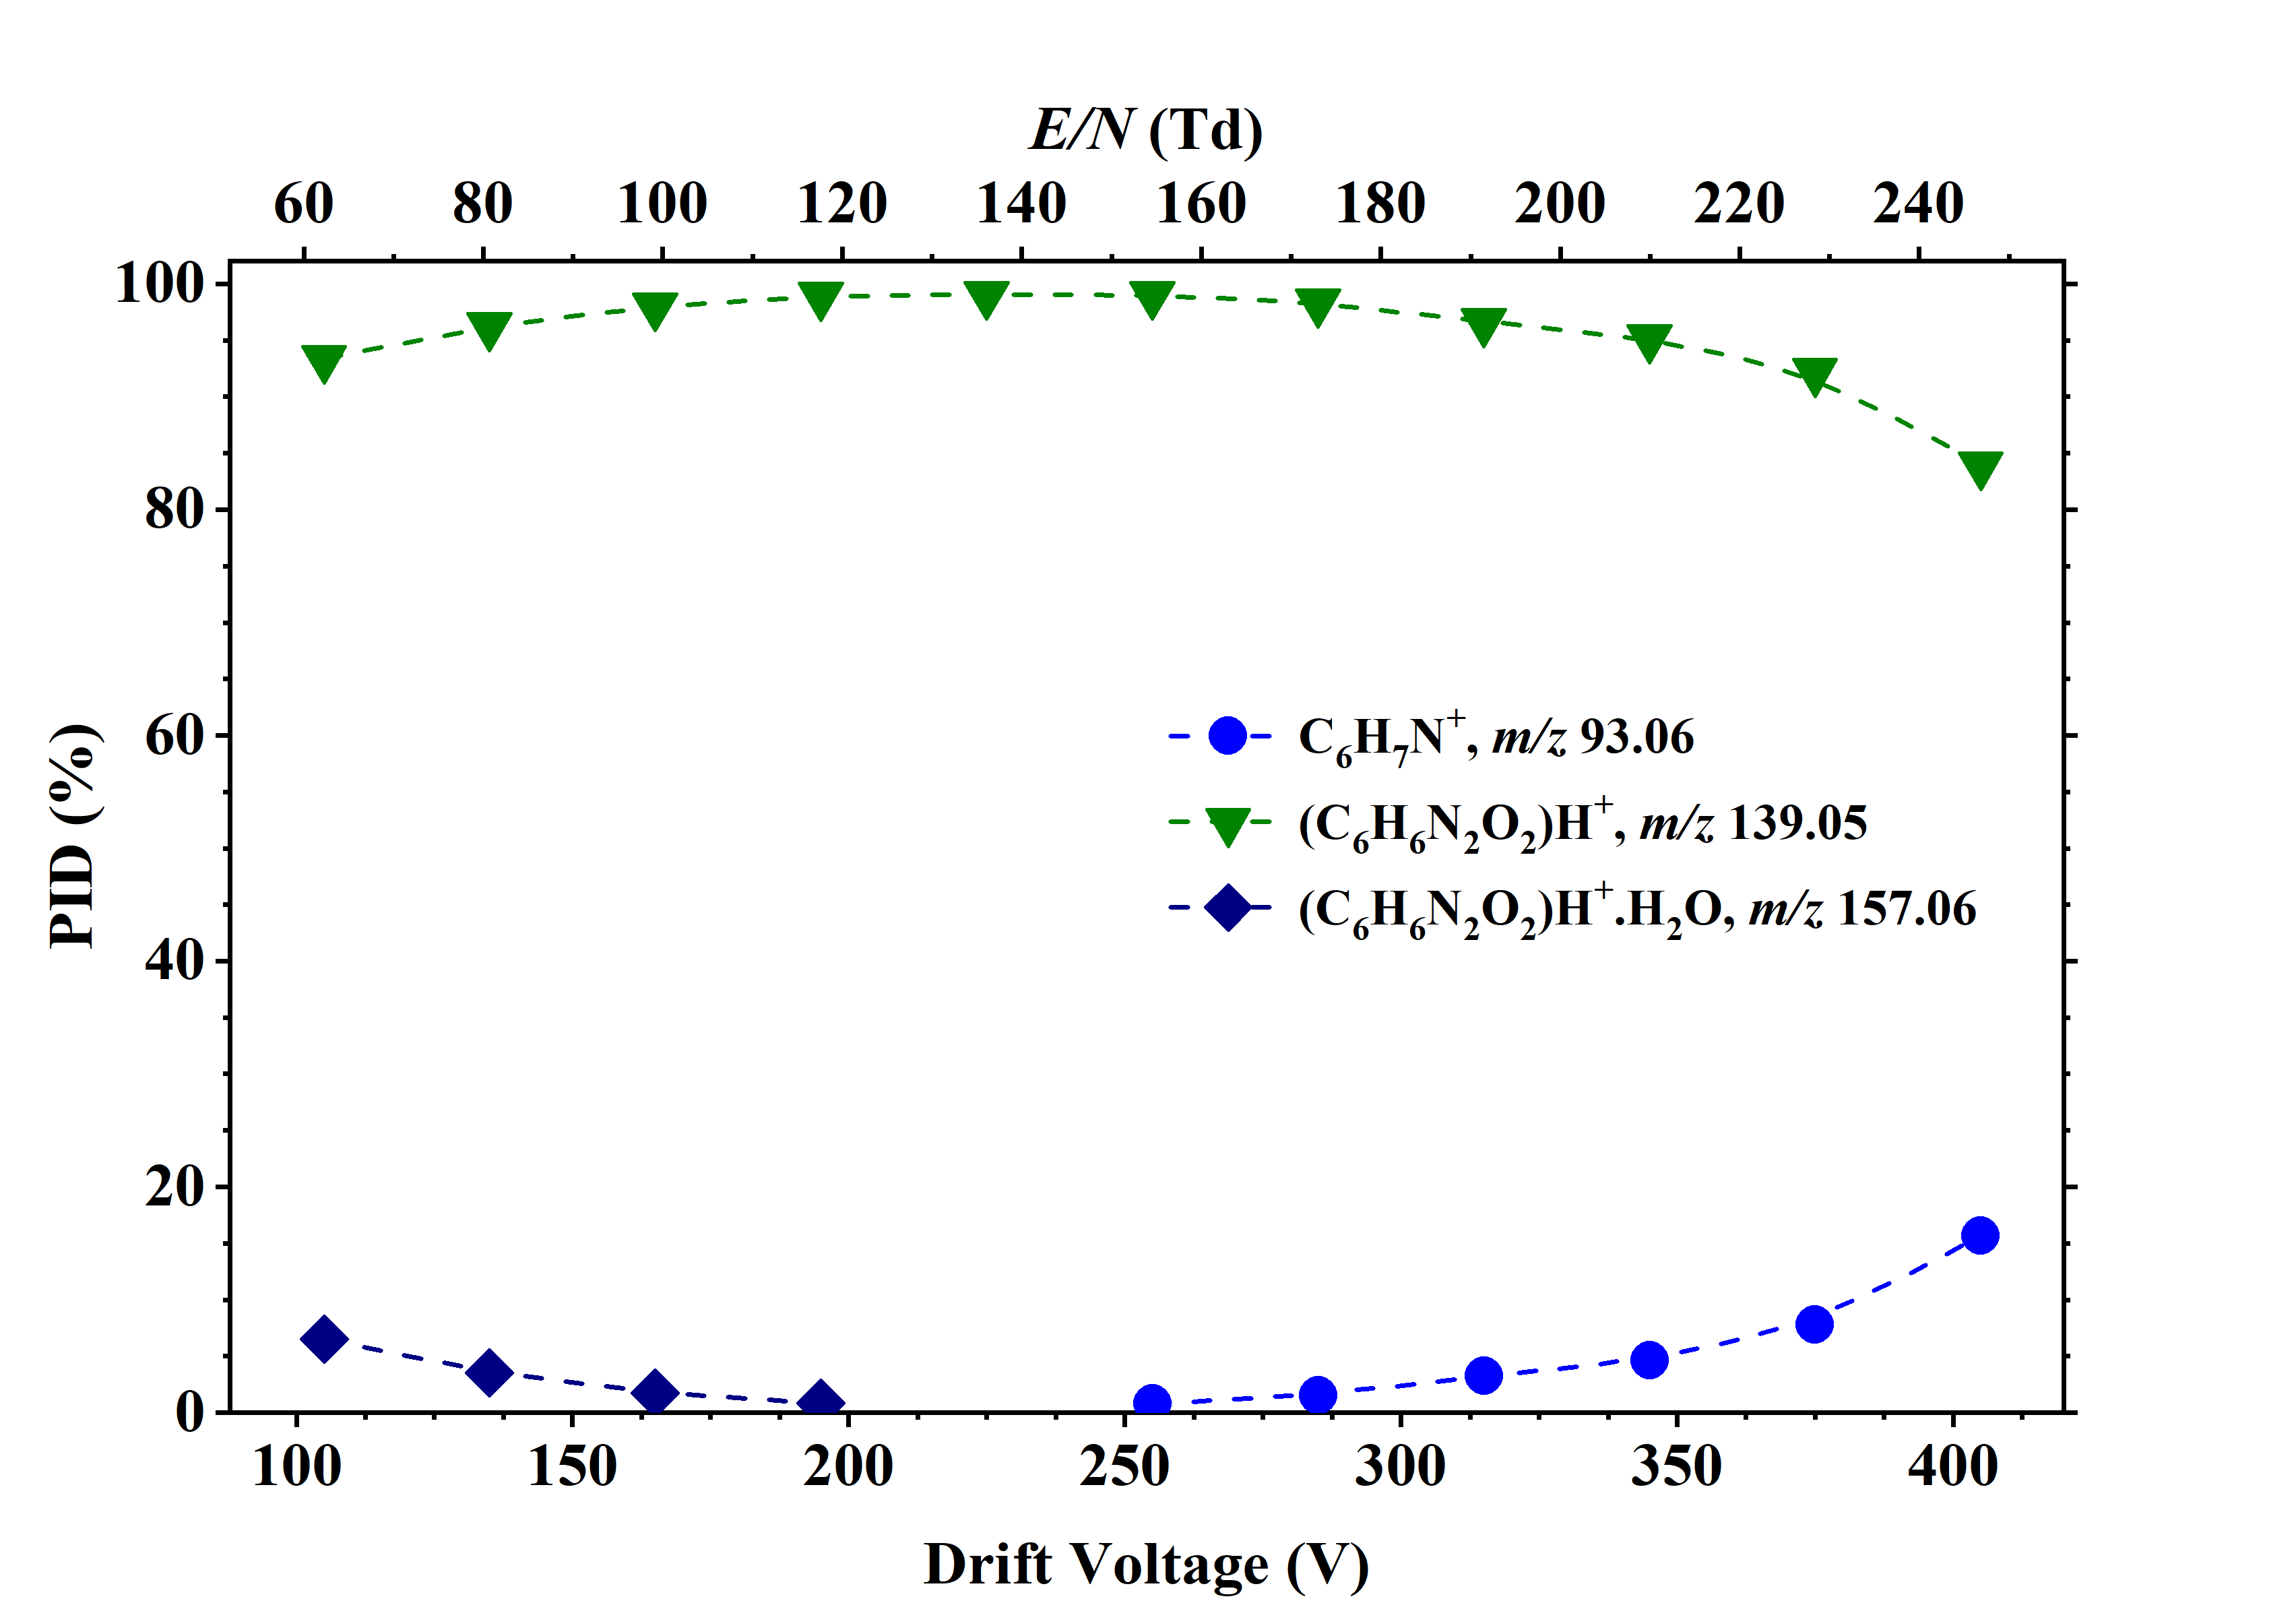
\includegraphics[height=0.35\textheight]{pics/nitros_paper_5.png}
\caption{Percentage product ion distribution resulting from the reaction of 4-nitroaniline with H$_3$O$^+$.(H$_2$O)$_n$ (n = 0, 1, 2) as a function of the reduced electric field from 60 to 250 Td.}
\label{fig:na_fig5}
\end{figure}

\subsection{Fragmentation patterns and branching percentage studies in charge transfer mode}

\subsubsection{2-nitroaniline}
The PID plot resulting from the reaction of 2-nitroaniline with O$_2^+$ as a function of the \textit{E/N} is shown in  \autoref{fig:na_fig6}.
The charge-transferred parent ion 2-NA$^+$ at \textit{m/z} 138.04 is the most abundant ion below 230 Td.
The branching percentage of this ion decreases with the \textit{E/N} while other product ion arise, with C$_5$H$_6$N$^+$ at \textit{m/z} 80.05 becoming dominant at 230 Td. 
The other observed fragment ions, in order of increasing \textit{m/z} are C$_5$H$_5^+$ at \textit{m/z} 65.04, 
the loss of the nitro group from 2-NA$^+$ (i.e. C$_6$H$_6$N$^+$) at \textit{m/z} 92.05 and
the loss of NO from 2-NA$^+$ (i.e. C$_6$H$_6$NO$^+$) at \textit{m/z} 108.04.
All these product ions have been reported by \citeauthor{beynon1959some} for electron impact experiments   \cite{beynon1959some}.

%\autoref{fig:na_fig6} presents a summary of the results for the reaction of O$_2^+$ with 2-NA as a function of reduced electric field. The parent ion at \textit{m/z} 138.04, [2-NA]+, resulting from non-dissociative charge transfer, dominates up to about 230 Td.  Its abundance decreases as the reduced electric field increases, and at \textit{E/N} above ca. 230 Td, \textit{m/z} 80.05 (assigned to the product ion C$_5$H$_6$N$^+$) becomes dominant. Other product ions, resulting from dissociative charge transfer, are observed at \textit{m/z} 65.04 (C$_5$H$_5^+$), \textit{m/z} 92.07 (C$_6$H$_6$N$^+$) (loss of NO$_2$) , \textit{m/z} 108.04 (C$_6$H$_6$NO$^+$) (loss of NO) and \textit{m/z} 121.04 (C$_6$H$_5$N$_2$O$^+$) (loss of OH). C$_6$H$_5$N$_2$O$^+$ was not observed in any of the other isomers. 

\begin{figure}%[h]
\centering
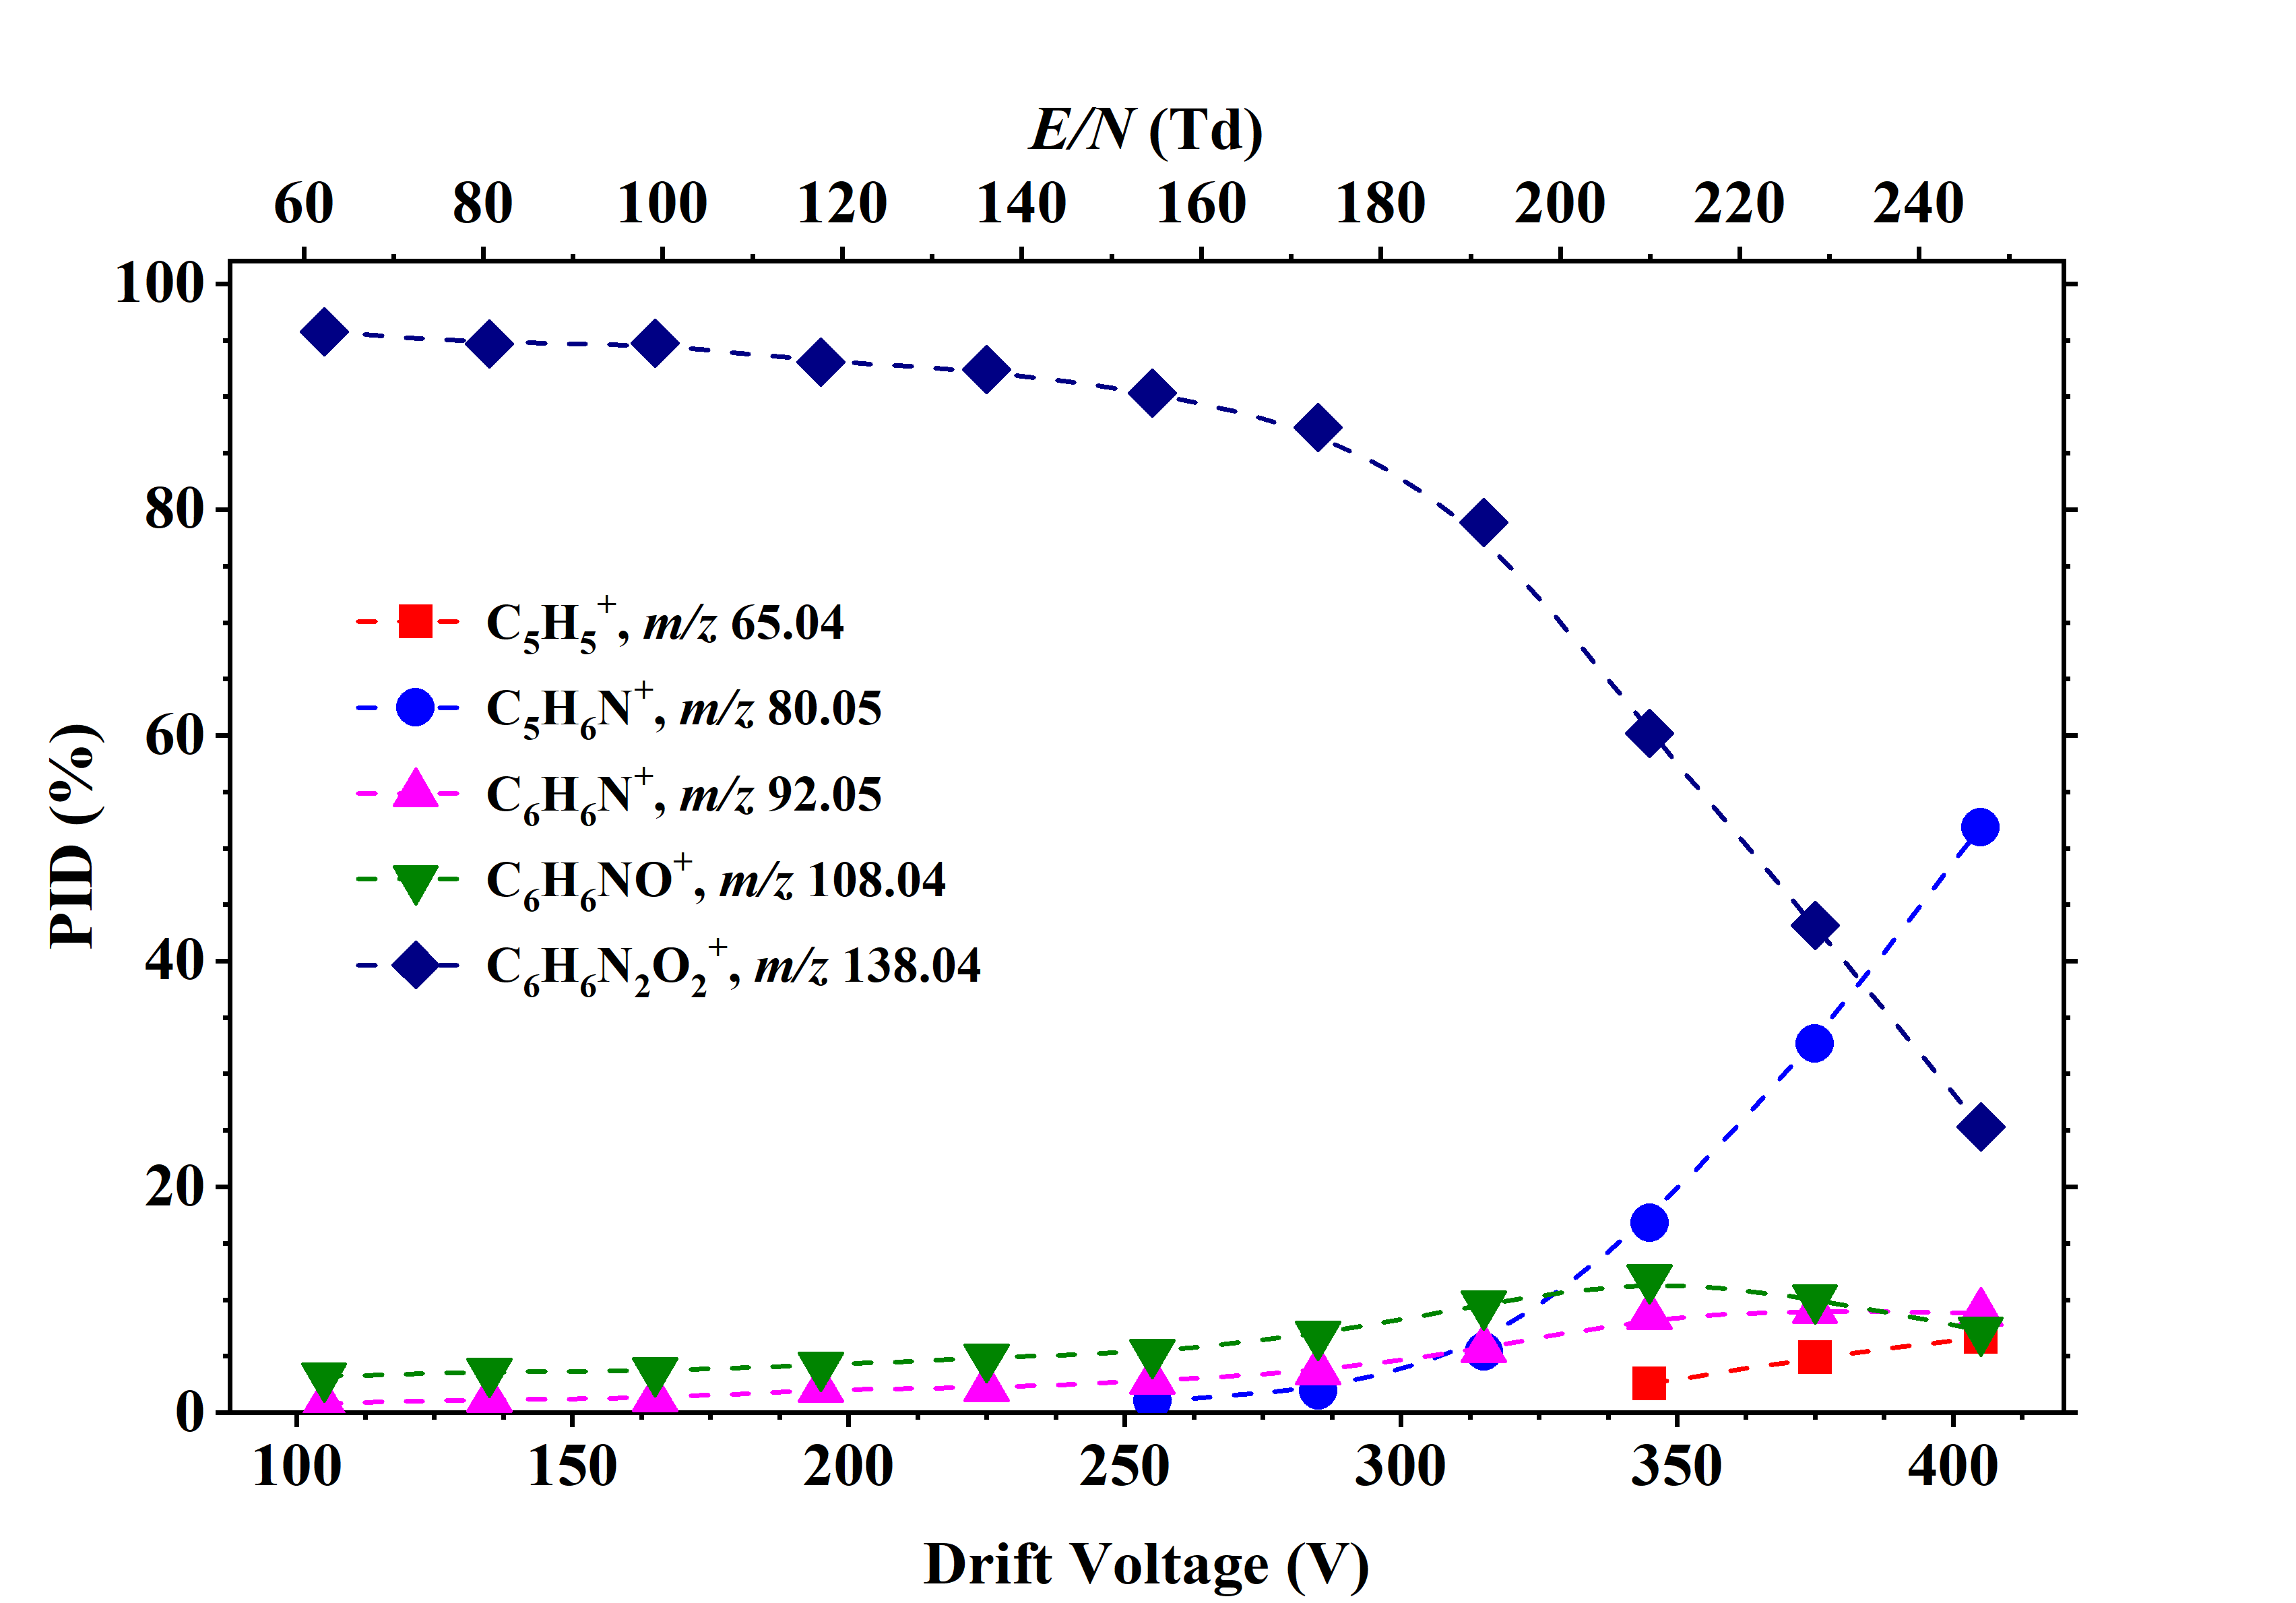
\includegraphics[height=0.35\textheight]{pics/nitros_paper_6.png}
\caption{Percentage product ion distribution  resulting from the reaction of 2-nitroaniline with O$_2^+$ as a function of the reduced electric field from 60 to 250 Td.}
\label{fig:na_fig6}
\end{figure}


\subsubsection{3-nitroaniline}
\autoref{fig:na_fig7} shows the PID plots for the reaction of 3-nitroaniline with O$_2^+$ as a function of the reduced electric field, which is quite similar to that of the 2- isomer in \autoref{fig:na_fig6}.
The observed product ions correspond to the same structures as indicated in the previous section, being in this case 3-NA$^+$ the parent ionised molecule.
However, their branching percentages for a given \textit{E/N} is slightly different.
For the 3- isomer, the parent ion is the most abundant over the whole reduced electric field study except for values higher than 240 Td, where C$_5$H$_6$N$^+$ at \textit{m/z} 80.05 becomes dominant.
Also, C$_6$H$_6$N$^+$ at \textit{m/z} 92.05 reaches a maximum product ion distribution of 15\% for 3-NA, while only around 5\% for 2-NA, and for C$_5$H$_5^+$ at \textit{m/z} 65.04 it is 12\% for 3-NA and around 6\% for 2-NA.
%For 3-NA a very similar fragmentation product ion pattern found for that of 2-NA is observed, as shown in \autoref{fig:na_fig7}. Products ions are observed at \textit{m/z} \textit{m/z} 65.04 (C$_5$H$_5^+$), 80.05 (C$_5$H$_6$N$^+$), \textit{m/z} 92.07 (C$_6$H$_6$N$^+$), \textit{m/z} 108.04 (C$_6$H$_6$NO$^+$), and \textit{m/z} 138.04, [3-NA]+, but with slight differences in their intensities at very high \textit{E/N} values. For 3-NA, the parent ion at \textit{m/z} 138.04, [3-NA]$^+$dominates for most of the reduced electric field investigated. But by about 240 \textit{m/z} 80.05 (C$_5$H$_6$N$^+$) becomes dominant. A clear difference is the intensity for the product ion at \textit{m/z} 92.05 (C$_6$H$_6$N$^+$), going up to ca. 15\% (compared to only ca. 5\% for 2-NA) and at \textit{m/z} 65.04 (C$_5$H$_5^+$) (ca. 12\% for 3-NA compared to ca. 6\% for 2-NA). 


\begin{figure}%[h]
\centering
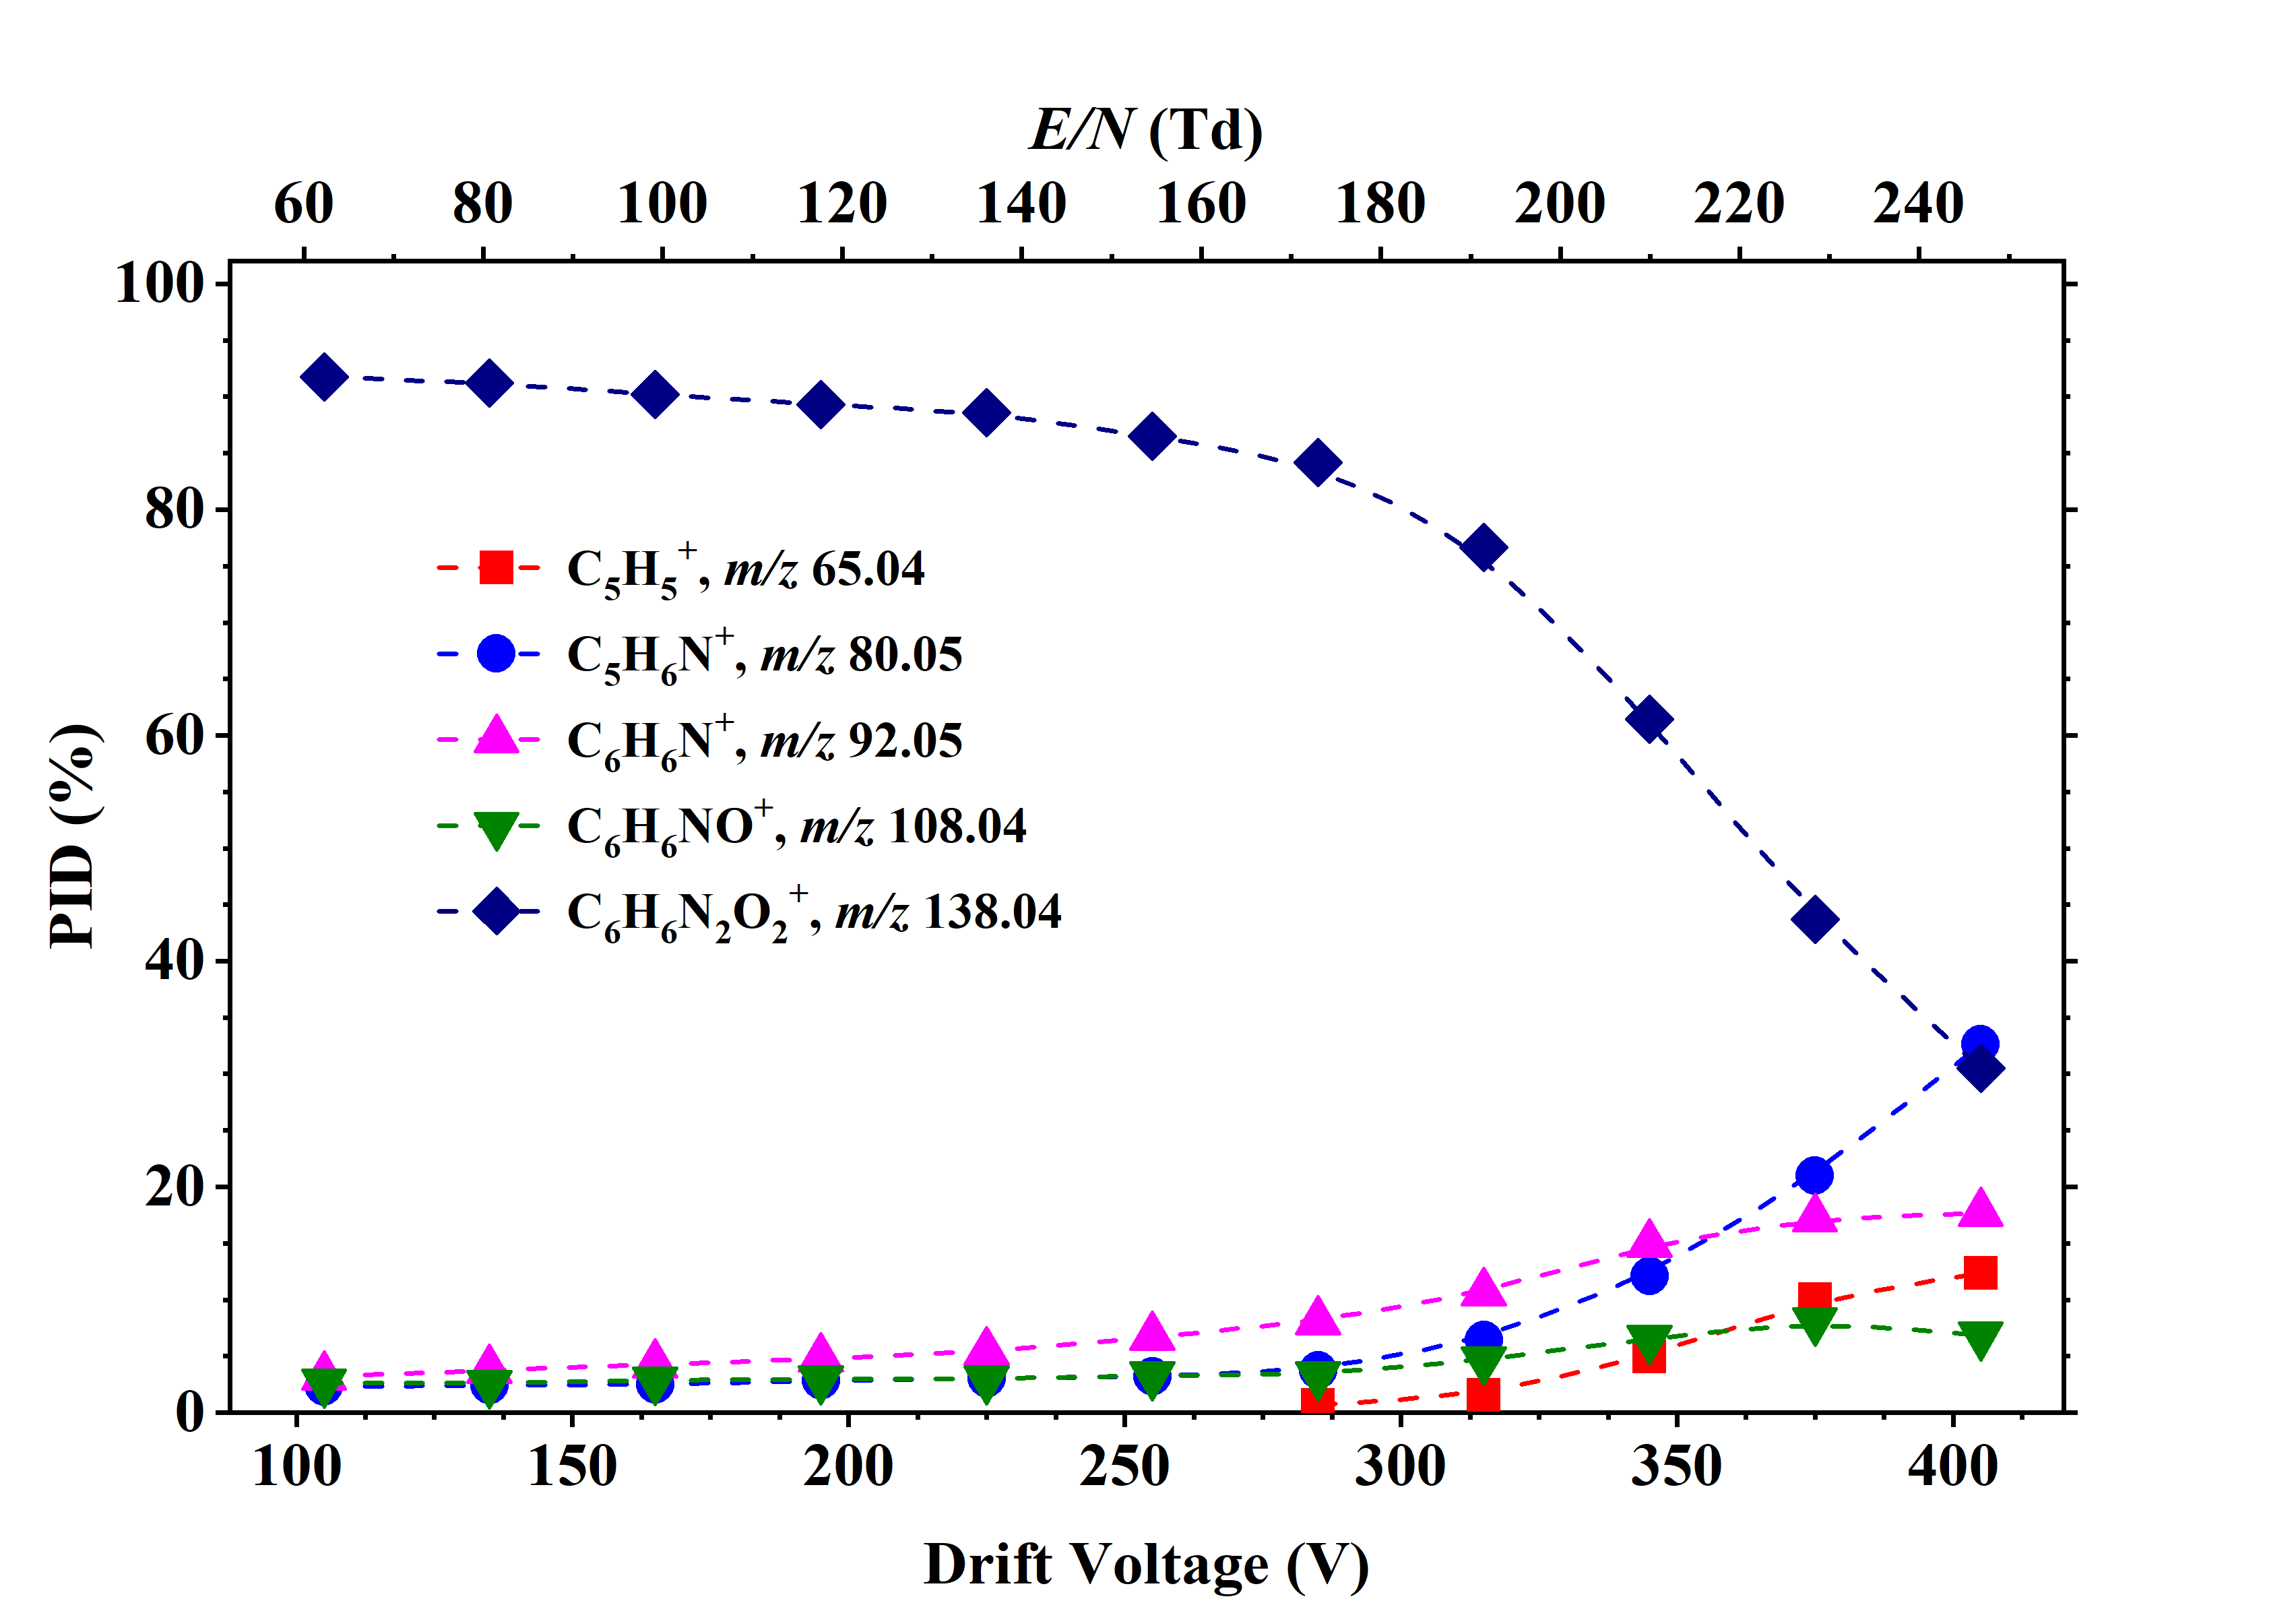
\includegraphics[height=0.35\textheight]{pics/nitros_paper_7.png}
\caption{Percentage product ion distribution resulting from the reaction of 3-nitroaniline with O$_2^+$ as a function of the reduced electric field from 60 to 250 Td.}
\label{fig:na_fig7}
\end{figure}


\subsubsection{4-nitroaniline}
The PID plot in \autoref{fig:na_fig8} shows that the fragmentation for 4-NA is different to that for the 3- and 2- isomers showing only three product ions.  
As stated in the proton transfer mode case, this is an effect coming from the \textit{para} arrangement of the functional groups in the ring.
For the 4-nitroaniline isomer, the parent ion (4-NA$^+$ at \textit{m/z} 138.04) is the most abundant from low reduced electric field up to around 190 Td, where C$_6$H$_6$NO$^+$ at \textit{m/z} 108.04 becomes dominant.
Furthermore, C$_5$H$_6$N$^+$ at \textit{m/z} 80.05 appears at 190 Td and increases with the \textit{E/N}, reaching a branching percentage of around 30\% at 250 Td.
%The product ion fragmentation pattern for 4-NA, as shown in \autoref{fig:na_fig8}, is very different from that observed for the other two isomers, with a simpler product ion distribution being observed, having only three product ions. This is a direct consequence of the para position for the substituents in the aromatic ring. The parent ion at \textit{m/z} 138.04, [4-NA]+, dominates from 60 Td up to ca. 190 Td, after which the product ion at \textit{m/z} 108.04 (C$_6$H$_6$NO$^+$) becomes dominant. For \textit{E/N} values above 190 Td, another fragment ion at \textit{m/z} 80.05 (C$_5$H$_6$N$^+$) becomes relevant, having a maximum intensity of ca. 30\% at an \textit{E/N} value of 250 Td.

\begin{figure}%[H]
\centering
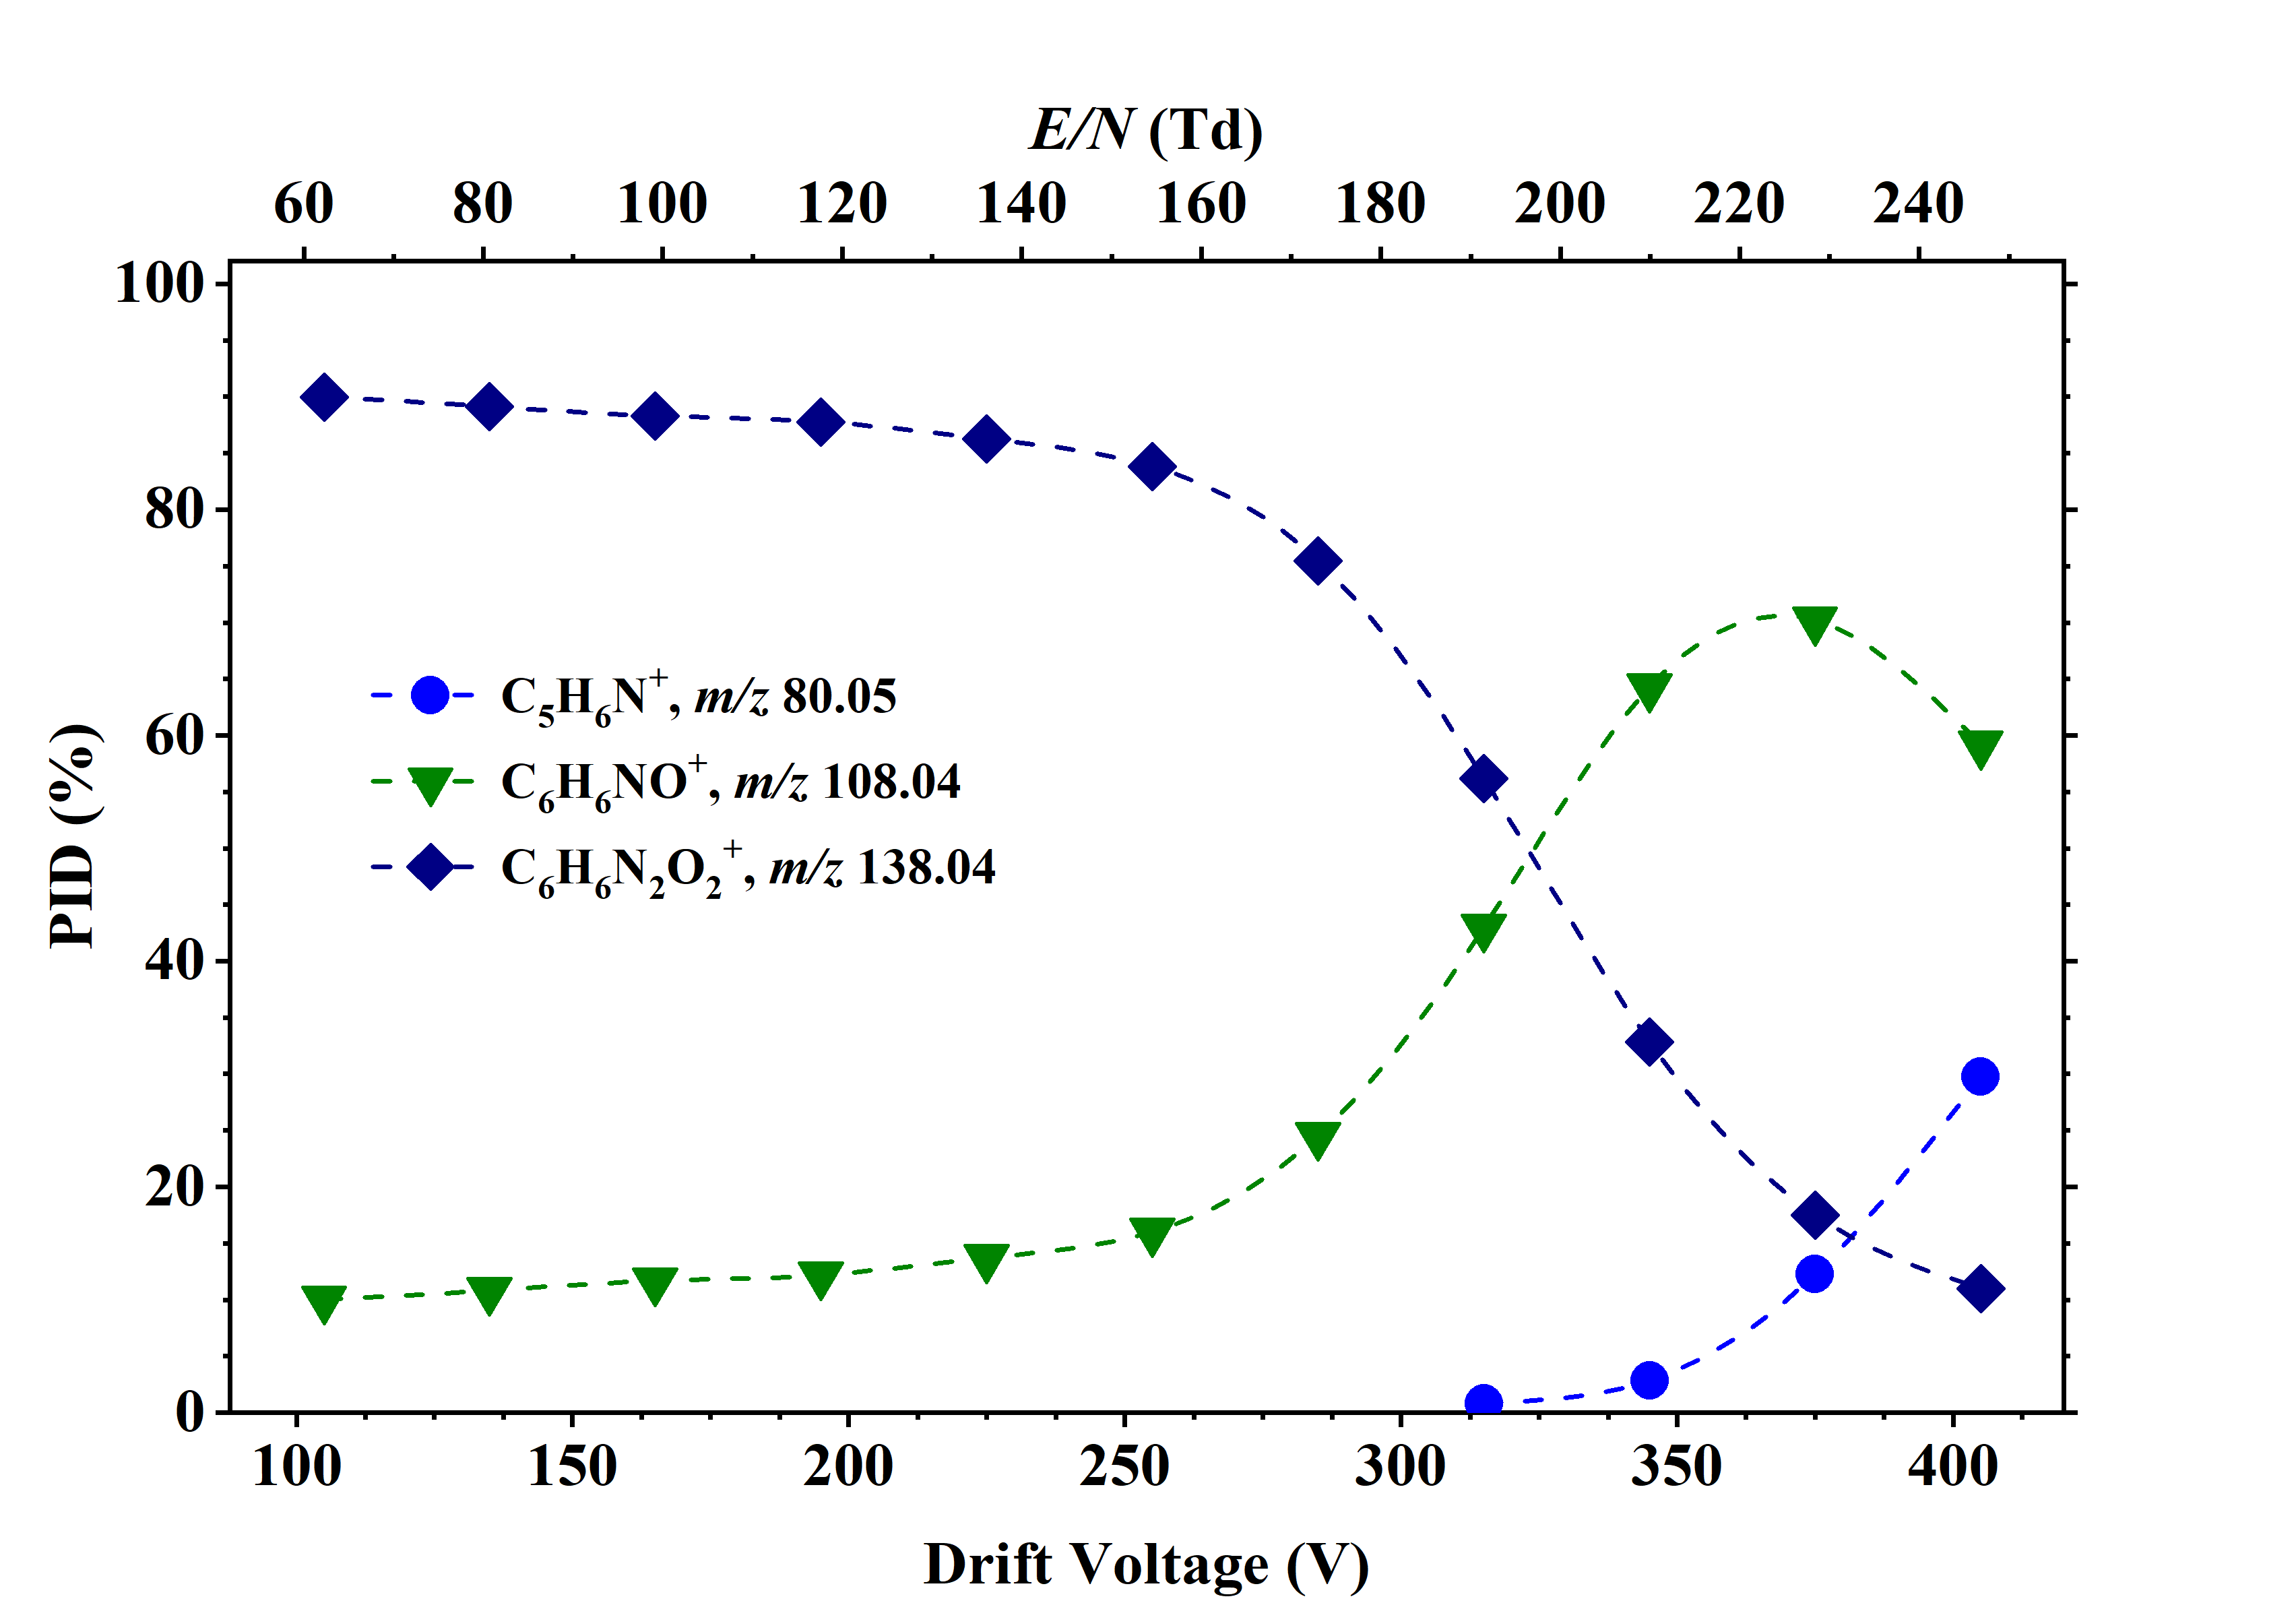
\includegraphics[height=0.35\textheight]{pics/nitros_paper_8.png}
\caption{Percentage product ion distribution resulting from the reaction of 4-nitroaniline with O$_2^+$ as a function of the reduced electric field from 60 to 250 Td.}
\label{fig:na_fig8}
\end{figure}


\section{Conclusions}
With this investigation we have shown how to separate nitroaniline isomers using the SRI-MS technique to enhance the ion/molecule reactions. This study contains the product ion distributions resulting from the reaction of the three isomers with H$_3$O$^+$ and O$_2^+$ as a function of the reduced electric field illustrated with quantum chemical results. 
We have proved that SRI-MS has good selectivity when detecting nitroanilines with H$_3$O$^+$ and O$_2^+$ as reagent ions. 

In the proton transfer mode, the protonated parent at \textit{m/z} 139.05 was the dominant ion over a wide \textit{E/N} range for the three nitroanilines, while for the charge transfer mode the parent ion at \textit{m/z} 138.04 was the most abundant for almost the whole \textit{E/N} range.
It is however the clustering with water in proton transfer mode and the presence of the product ion at \textit{m/z} 108.04 in charge transfer mode what allows for isomer identification here. 
Whilst the product ion distributions of the reactions of 2- and 3-nitroaniline with O$_2^+$ are very similar, the 3- isomer shows higher clustering with water at low \textit{E/N} in proton transfer mode, with the 3-NA.H$^+$.H$_2$O ion reaching ca. 50\% at 60 Td (i.e. the lowest reduced electric field). 
Moreover, 4-nitroaniline shows less fragmentation than the 2- and 3- isomers in proton transfer mode but, in charge transfer mode, C$_6$H$_6$NO$^+$ at \textit{m/z} 108.04 becomes the most abundant ion above approximately 190 Td. 
This ion enables the identification of the 4- isomer, as it never represents more than about 15\% for 2- or 3-nitroaniline.
%This work reports the product ions from the reaction of 2-, 3- and 4-nitroaniline isomers with H$_3$O$^+$ and O$_2^+$ as a function of the reduced electric field in a SRI-ToF-MS. We have shown that selective reagent ion mass spectrometry, using either water or oxygen as reagent gases, can be used to detect nitroaniline isomers with good selectivity. The most abundant product ion for all the isomers for the reactions with H$_3$O$^+$ is the protonated parent at \textit{m/z} 139.05 over an extended reduced electric field range. For the reactions with O$_2^+$, non-dissociative charge transfer results in the parent ion at \textit{m/z} 138.04 being the most abundant product ion. However, relative ion abundances are different for each reagent ion. 2- and 3-NA show very similar fragmentation patterns with O$_2^+$, while with H$_3$O$^+$, 2-NA shows smaller water clustering at low \textit{E/N} and its fragment product ions become dominant at a lower \textit{E/N} than found for 3-NA. 4-NA shows less fragmentation with H$_3$O$^+$, and for the reaction with O$_2^+$ a distinctive fragment ion is observed at \textit{m/z} 108.04, which becomes dominant above about 190 Td. The presence or absence of this product ion at \textit{m/z} 108.04 easily allows for reliable identification of the 4-NA isomer. 

%This study demonstrates how it is possible to distinguish isomers based on the manipulation of the ion/molecule chemistry and/or using different reagent ions that favour different ionisation mechanisms. 


%\section{Acknowledgements}
%We thank the Marie Skłodowska-Curie Actions Innovative Training Network: Ion-Molecule Processes for Analytical Chemistry Technologies (IMPACT) (www.impact-h2020itn.com) which has supported this research through the European Commission’s HORIZON 2020 Programme under Grant Agreement Number 674911. DOL is an Early Stage Researcher on IMPACT. We also thank Dr. Peter Watts (a member of the Molecular Physics Group, School of Physics and Astronomy, University of Birmingham, UK) for undertaking the DFT calculations presented in this paper. The authors also thank Mahroz Mirzahekmati for producing the graphical abstract.































































